\documentclass[12pt]{article}

% This is the latex file to provide extra support for the statistical
% analyses for the lab portion of the class.
%
% It is written by
%    Kelly Black and
%    Leah Ziamandanis
%

%
% $Author: black $
% $Date: 2007/03/27 19:01:35 $
% $RCSfile: experimental.tex,v $
% $Revision: 1.52 $
%
%

\def\solutions{y}
\def\solutions{n}




\ifx\pdfoutput\undefined
\usepackage{graphicx}
\usepackage{geometry}
\usepackage{color}
\else
\usepackage[pdftex]{graphicx}
\usepackage[pdftex]{geometry}
\usepackage[pdftex]{color}
\usepackage{hyperref}
\hypersetup{
  pdftitle={Statistics Supplament for IMPS},
  pdfsubject={Experimental Statistics},
  pdfauthor={Kelly Black},
  pdfkeywords={Statistics},
  anchorcolor = {red},
  colorlinks = {true},
  %pdfpagemode={FullScreen}
}
\fi

\oddsidemargin=0.0in
\evensidemargin=0.0in
\textwidth=6.5in

\topmargin=-0.5in
\textheight=9in



\newtheorem{definition}{Definition}[section]
\newtheorem{example}{Example}[section]
\newtheorem{assignment}{Assignment}[section]
\newtheorem{theorem}{Theorem}[section]


\newcommand{\lp}{\left(}
\newcommand{\rp}{\right)}

\begin{document}

\begin{center}
  {\Large Brief Introduction to Statistics and Error Analysis
    for Experiments\footnote{
                 This work is licensed under the Creative Commons 
		 Attribution-NonCommercial-ShareAlike 2.5 License. 
		 To view a copy of this license, visit 
		 http://creativecommons.org/licenses/by-nc-sa/2.5/ 
		 or send a letter to Creative Commons, 543 Howard Street, 
		 5th Floor, San Francisco, California, 94105, USA.}} \\
  Kelly Black and Leah Ziamandanis \\
  Department of Mathematics, Union College \\
  Summer 2006 \\
\if y\solutions
\textbf{Solution Manual}
\fi
\end{center}



\tableofcontents




\clearpage

\section{Introduction}

This is a basic overview of statistics and error analysis for
experiments. This is not an exhaustive treatment of the subject but
provides a broad introduction into the basic ideas. The first topic is
about error and how errors can be propagated in calculations.  Next,
the basic ideas about data and how to describe data are examined. Once
that is done a more formal approach to aid in the analysis of data is
examined, and a more formal description of error is given.  Finally, a
basic overview of how to fit straight lines to data is given.

This material is brief and many ideas and subtleties do not receive
the attention that they deserve. This is an introduction to an
important topic.  Experimental design, the practice of experimental
procedures, and the analysis of experimental data are nontrivial
topics that are closely linked. They are areas that are the subject of
intense study and a complete treatment is beyond the scope of a single
course.



\section{To Err is Human}

Every measured value in an experiment comes with an interval of
uncertainty, based on how accurate the value is expected to be.  It is
vital to pay careful attention to all possible uncertainties so that
the results in a lab can be reported in a fashion that is consistent
with the observations.  To define appropriate uncertainties for
measurements taken, all sources of error must be considered.  In many
cases, measurements are used to calculate other values, based on some
function.  The focus of this section is on how errors propagate
through calculations and uncertainties are carried past a given
function.

\subsection{Finding Appropriate Uncertainties}

For a direct measurement, like measuring length with a ruler for
example, the measurement will have an uncertainty based on the
measured increments of the instrument.  For example, suppose that
measuring the width of a paper clip in millimeters yields a value
between 2mm and 3mm, but there are no marks between each millimeter,
the experimenter can only be accurate up to half a millimeter.  So the
measured value should be recorded as $2.5\pm .5$ mm.  Other
instruments such as thermometers, protractors, and voltmeters suffer
from the same problem.  Every measured value, \textit{x}, includes
some uncertainty, $\triangle{x}$.  In the example with the paper clip
the uncertainty is $\triangle{x} = .5$mm.

The physical limit of a device may not represent the uncertainty of a
measurement in practice. As an example suppose that a timing
experiment is to be performed.  One student measures the time it takes
for a ball to hit the ground after dropping it from a predetermined
height, and the measured time is $5.2 \pm .1$s.  Another student
measures the time to be $6.4 \pm .1$s.  How can they both be correct?
It would seem that a time of $5.8 \pm .7$ sec.  would be a more
accurate representation of the actual time.  It is not always clear
what the actual uncertainty is in a measurement. \textit{For this
  reason, any measurement that can be repeated, should be repeated}.
The methods to determine the uncertainties for repeated measurements
are examined in Section \ref{sect:data}.


\subsection{Systematic Errors and Bias}

There are two other sources of error aside from errors in direct
measurements\cite[pp 12-89]{introErrorAnalysis}. One kind of error
occurs when it is not clear what event should be measured. The other
kind of error occurs when the measurement is consistently wrong. The
two kinds of error lead to the following definitions.

\begin{definition}
A \textbf{problem of definition} occurs
when it is not clear where the points to be measured exactly are.  A
problem of definition can be caused by physical obstacles, e.g. you
can't fit your ruler into a small space.  
\end{definition}

\begin{definition}
A \textbf{systematic error} is a circumstance or instrument that will
always push the measurement either high or low with every trial, e.g.
a clock that runs slow.  
\end{definition}

The experimenter must always consider every possible source of error,
including personal bias.  The expectation to obtain a certain value
must be eliminated.  That may be difficult if the value was found by
another scientist or because you would guess that it is correct, but
expectations must be disregarded\cite{Gould81}.

The basic issue is that an experimenter intends to make measurements
that are close to the true value. If a measurement is close to the
true value then the measurement is ``accurate.''  Unfortunately, a
measurement is taken because the true value is not known. 

It is important to note the difference between \textit{precision},
\textit{bias} and \textit {accuracy}.  A precise group of measurements
are relatively close to each other, but because of bias, they may be
skewed away from the actual answer.  An accurate set of measurements
are close to the true value.

An example of the difference is shown in Figure
\ref{fig:biasPrecision}. The example in panel A shows measurements
that are relatively precise but consistently biased to the right of
the true value. The measurements in A are not accurate. The example in
panel B show measurements that have a similar level of precision but
less bias. The measurements in B are accurate. The example in panel C
show measurements that are more tightly clustered around the true
value and are more precise with little bias. The measurements in C are
accurate. Finally, the example in panel D shows measurements with
little bias that have a large spread around the true value and are
less precise than the previous examples. The measurements in D are
accurate.

\begin{figure}[tb]
  \centerline{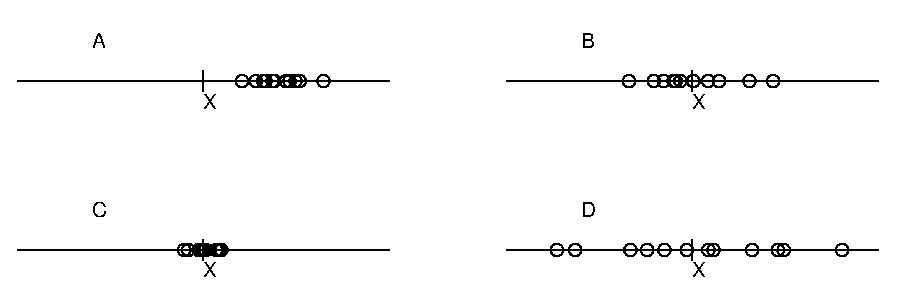
\includegraphics[width=4.5in]{bias}}
  \caption{Data is observed to verify that it is close to X. In plot A
    there is a bias away from X and in plot B the data is centered on
    X. In plot C the data is closely clustered close to X with small
    variance (high precision), and in plot D the data has larger
    variance (low precision).}
  \label{fig:biasPrecision}
\end{figure}


\subsection{Error Propagation}

In a laboratory, measured values are almost always utilized in
formulas providing useful findings for the experimenter.  After
calculations, a final answer cannot be left without uncertainty
considering that the measured values have uncertainties.  Once
measured values are paired with appropriate uncertainties the measured
values can be used in calculations and appropriate uncertainties can
be calculated for the new values.  The focus of this section is on the
mathematical tools that can be used to define how error propagates in
a series of calculations.
  
One simple example is calculating the difference between the
temperature yesterday and the temperature today.  How do the
uncertainties of each measurement affect the uncertainty in the final
answer?  More difficult questions about how error propagates in the
final product come with more advanced calculations.  Some simple
calculus provides rules that can be applied to any calculation given
an approximation of the uncertainty.

First, an example of calculating uncertainties using a longer, more
difficult technique is considered as a way of motivating the issues.
The goal is to find the uncertainty in calculating the product $x
\cdot y$ for some measured values $x$ and $y$, along with
uncertainties $\triangle{x}$ and $\triangle{y}$.  

To compute the value of their product, $f(x,y)~=~x\cdot y$,
abbreviated as $f~=~x\cdot y$, a value for $\triangle{f}$ must be
found.  But what is an appropriate value for $\triangle{f}$?
Considering the uncertainties for $x$ and $y$, the biggest and
smallest possible values for $f$ using the extreme possible values of
$x$ and $y$ can be found:
\begin{eqnarray}
f_\mathrm{big} &=& (x~+~\triangle{x})(y~+~\triangle{y}), \\
f_\mathrm{small} &=& (x~-~\triangle{x})(y~-~\triangle{y}).
\end{eqnarray}
At the same time the range of values of $f$ can be written in terms of
$\triangle f$,
\begin{eqnarray}
f_\mathrm{big} &=& (f~+~\triangle{f}), \\
f_\mathrm{small} &=& (f~-~\triangle{f}).
\end{eqnarray}

Subtracting the two equations yields
\begin{eqnarray}
f_\mathrm{big} - f_\mathrm{small} &=& 
(x + \triangle{x})(y + \triangle{y}) - 
(x - \triangle{x})(y - \triangle{y}), \\
&=& 2 \triangle{x} \cdot y + 2 x \cdot \triangle{y}.
\end{eqnarray}
The difference, $f_\mathrm{big}~-~f_\mathrm{small} = 2\triangle{f}$,
represents the uncertainty in the calculation of $f$, 
\begin{eqnarray}
\triangle{f} &=& \triangle{x} \cdot y~+~x \cdot \triangle{y}.
\end{eqnarray}
The calculation can be expressed with appropriate uncertainty,
\begin{eqnarray}
f &=& xy \pm (\triangle{x} \cdot y~+~x \cdot \triangle{y}).
\end{eqnarray}


This process can be too complicated for most other functions.
Fortunately, the value of $\triangle{f}$ can be approximated in an
easier fashion using a straight line approximation.  First a graphical
interpretation is examined.  Consider a measured value $x$ along with
an uncertainty $\triangle{x}$.  The value of $x$ is used to calculate
a new value, $f(x)$, as is shown on Figure \ref {fig:slopeError}.  

The best estimate for the value $f$ is $f(x)$, and to find how
$\triangle{x}$ propagates through the function $f$ a straight line
approximation is used.  The largest probable value of $x$ is
$x+\triangle{x}$, and from the graph the value $f+\triangle{f}$ is
approximately $f+\frac{df}{dx}\triangle x$.  Similarly the smallest
probable value of $x$ is $x-\triangle{x}$, and from the graph the
value $f-\triangle{f}$ is approximately $f-\frac{df}{dx}\triangle x$.
 
\begin{figure}[tb]
  \centerline{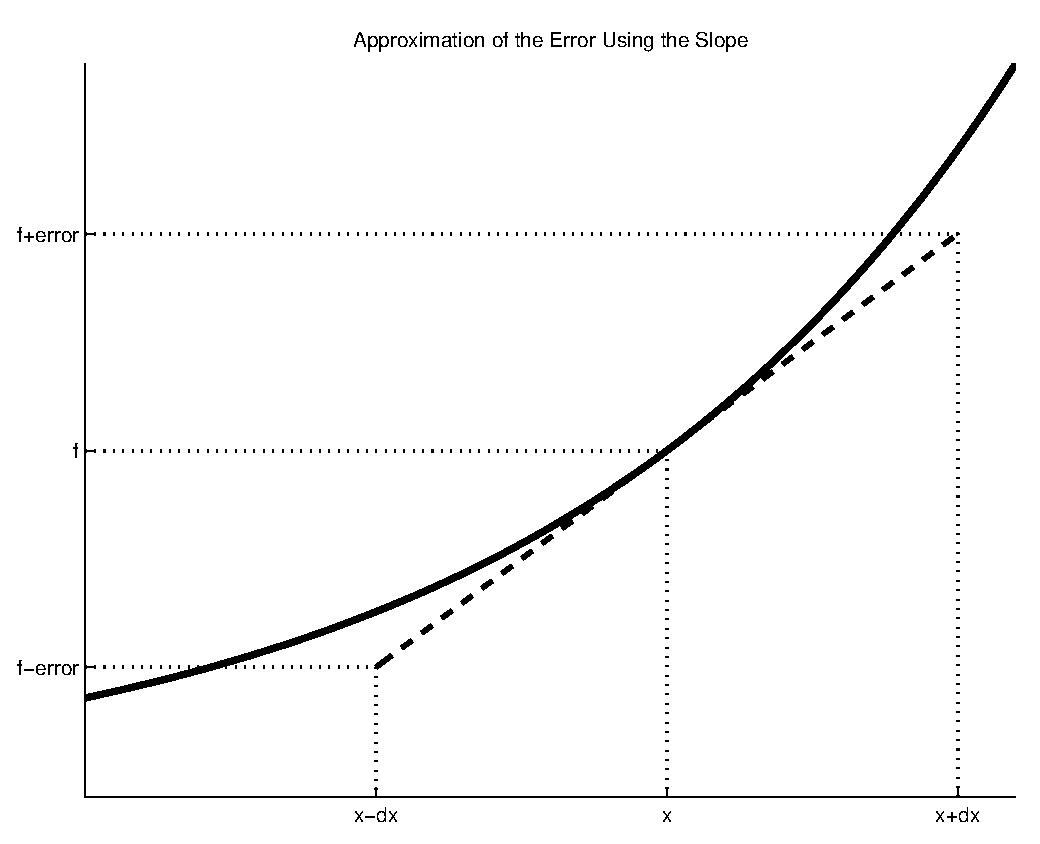
\includegraphics[height=3in]{slopeError}} %,angle=270
  \caption{The slope of the curve can be used to approximate the error
  at a point.}
  \label{fig:slopeError}
\end{figure}

From the graph an approximation for the change in the function is
\begin{eqnarray*}
\triangle{f} & = & f(x~+~\triangle{x})-f(x).  
\end{eqnarray*}
The linear approximation implies that for a small change, $\triangle
x$, 
\begin{eqnarray}
\triangle{f} & = & f(x+\triangle {x})-f(x), \\
& \approx & \frac{df}{dx}\triangle{x}.
\end{eqnarray}
This can be generalized for functions of more than one variable,
$f(x,\cdots,z)$ by
\begin{eqnarray}
  \triangle{f} & \approx & 
  \frac{\partial f}{\partial x}\triangle{x}
  +~\frac{\partial f}{\partial y}\triangle{y}
  +~\cdots~+\frac{\partial f}{\partial z}\triangle{z}.
\end{eqnarray}
 
 
Keep in mind that this is an approximation of the error, since the
function is not always a straight line (as shown in Figure
\ref{fig:slopeError}), but for small uncertainties it is close.
Revisiting a prior example, the error for $f(x,y)=x\cdot y$ is
approximated by applying the new derivative rule,
\begin{eqnarray}
 \triangle{f} &\approx& \frac{\partial f}{\partial x}\triangle{x}
 +\frac{\partial f}{\partial y}\triangle{y}, \\
 &=& y \cdot \triangle{x}+x \cdot \triangle{y},
\end{eqnarray}
which is the same value calculated earlier for $\triangle{f}$.  

Making use of the derivative to calculate the uncertainties is a
relatively straight forward procedure, but there is a problem with
this computed value for $\triangle{f}$.  The numerical values of the
errors may be negative and the final number may not make sense.
Another way to think about it is if each variable represents an error
in different, perpendicular directions, the $x$-direction and the
$y$-direction, see Figure \ref{fig:errorCircle}.  The error is better
approximated as the hypotenuse of a triangle,
\begin{eqnarray}
  \triangle{f}~=~\sqrt{\left(\frac{\partial f}{\partial x}\triangle{x}\right)^2
    +~\cdots ~+\left(\frac{\partial f}{\partial z}\triangle{z}\right)^2}.
\end{eqnarray}


\begin{figure}[tb]
  \begin{center}
    \begin{picture}(250,80)
      \put(10,20){\vector(1,0){220}}
      \put(230,20){\vector(0,1){52}}
      \put(10,20){\vector(4,1){217}}
      \put(120,5){$\frac{\partial f}{\partial x}\,\triangle x$}
      \put(235,42){$\frac{\partial f}{\partial y}\,\triangle y$}
      \put(35,65){$\sqrt{
        \lp\frac{\partial f}{\partial x}\,\triangle x\rp^2 + 
        \lp\frac{\partial f}{\partial y}\,\triangle y\rp^2}$}
    \put(10,20){\circle*{5}}
    \put(230,75){\circle*{5}}
    \put(0,5){\textit{Measured}}
    \put(237,75){\textit{Measured+Error}}
    \end{picture}
  \end{center}
  \caption{The difference between the true value and the measured
    value. The error in the $x$-direction is $\frac{\partial
      f}{\partial x}\,\triangle x$, and the error in the $y$-direction
    is $\frac{\partial f}{\partial y}\,\triangle y$. The total error
    can be approximated using the square root of the sum of the
    squares. }
  \label{fig:errorCircle}
\end{figure}




\begin{example}
  A cart of length $l$, rolling down a frictionless incline
  at an angle $\theta$ as shown in Figure \ref{fig:cartIncline}.  The
  expected acceleration of the cart is $g\sin(\theta)$, but the actual
  acceleration can be found when two photocells are placed with a
  measured distance, $s$, between them on the incline. The cart trips
  the photocell at the instant its front end passes the eye, and then
  trips again when the back end of the cart clears the cell.
  The following measurements are made during the experiment:
  \begin{eqnarray*}
    l & = & .10m~\pm~.01m, \\
    \theta & = & 0.45~\mathrm{rad.}~\pm~.02~rad., \\
    t_1 & = & .053~\mathrm{sec}~\pm~.001~sec, \\
    t_2 & = & .021~\mathrm{sec}~\pm~.001~sec, \\ 
    s & = & 2.3\mathrm{m}~\pm~.1m. 
  \end{eqnarray*}
\end{example}

If the cart takes $t_1$ sec.  to pass the first photocell, then its
speed is, $v_1~=~\frac {l}{t_1}$.  If the cart takes $t_2$ sec.  to
pass the second photocell, then its speed is, $v_2~=~\frac{l}{t_2}$.
($v_1$ and $v_2$ are average speeds, but if l is small then the
instantaneous speeds are close to the average speeds).  Now, if the
distance between the photocells is s, then the formula
${v_2}^2~=~{v_1}^2~+~2as$ gives
\begin{eqnarray*}
  a &=& \frac{{v_2}^2~-~{v_1}^2}{2s}, \\
    &=& \left( \frac{l^2}{2s} \right) 
      \left( \frac{1}{{t_2}^2}~-~\frac{1}{{t_1}^2} \right).
\end{eqnarray*}
Using this equation, $a$ can be found along with its error $\triangle{a}$. \\


The best approximation for the acceleration is,
\begin{eqnarray*}
 a & = & \lp\frac{l^2}{2s}\rp
       \lp\frac{1}{{t_2}^2}~-~\frac{1}{{t_1}^2}\rp, \\
   & \approx & \lp\frac{.1^2}{2(2.3)}\rp
               \lp\frac{1}{{.021}^2}~-~\frac{1}{{.053}^2}\rp, \\
   & \approx & 4.156~\mathrm{m/sec}^2.
\end{eqnarray*}

To find $\triangle{a}$, first find the amount each individual variable
contributes to the uncertainty:
\begin{eqnarray*}
\frac{\partial a}{\partial l}~&=&~\left(\frac{l}{s}\right)\left(\frac{1}{{t_2}^2}~-~\frac{1}{{t_1}^2}\right)~=~
\left(\frac{.1}{2.3}\right)\left(\frac{1}{.021^2}~-~\frac{1}{.053^2}\right)~\approx~83.11  \\
\frac{\partial a}{\partial s}~&=&~\left(\frac{-l^2}{2s^2}\right)\left(\frac{1}{{t_2}^2}~-~\frac{1}{{t_1}^2}\right)~=~\left(\frac{-(.1^2)}{2(2.3^2)}\right)\left(\frac{1}{.021^2}~-~\frac{1}{.053^2}\right)~\approx~1.81    \\
\frac{\partial a}{\partial t_1}~&=&~\frac{l^2}{s({t_2}^3)}~=~\frac{.1^2}{2.3(.053^3)}~\approx~29.20   \\
\frac{\partial a}{\partial t_2}~&=&~\frac{-l^2}{s({t_2}^3)}~=~\frac{-(.1^2)}{2.3(.021^3)}~\approx~-469.48.
\end{eqnarray*}
Then substitute these values into the uncertainty formula previously derived:
\begin{eqnarray*}
\triangle{a} & = & \sqrt{
   \lp\frac{\partial a}{\partial l}\triangle{l}\rp^2 +
   \lp\frac{\partial a}{\partial s}\triangle{s}\rp^2 +
   \lp\frac{\partial a}{\partial t_1}\triangle{t_1}\rp^2 +
   \lp\frac{\partial a}{\partial t_2}\triangle{t_2}\rp^2 }, \\
 & \approx & \sqrt{
   \lp 83.11\cdot.01 \rp^2 + \lp 1.81\cdot.1 \rp^2 + \lp 29.20\cdot.001 \rp^2 +
   \lp -469.48\cdot.001 \rp^2}, \\
 & \approx & 0.972 ~ \mathrm{m/sec}^2.
\end{eqnarray*}
The calculation of the acceleration is $a~=~4.~\pm~1. ~ \mathrm{m/sec}^2$.

\begin{figure}[tb]
  \centerline{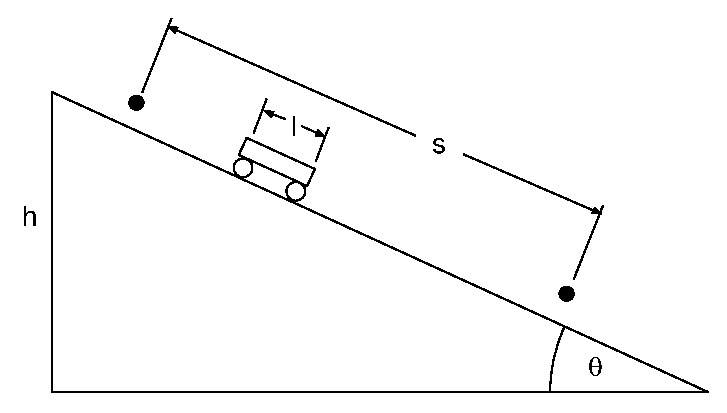
\includegraphics[width=3in]{incline-1}}
  \caption{The cart is moving down an incline plane with height $h$
    and angle $\theta$. The photocells are a distance $s$ apart, and
    the cart has length $l$.}
  \label{fig:cartIncline}
\end{figure}

\begin{figure}[tb]
  \centerline{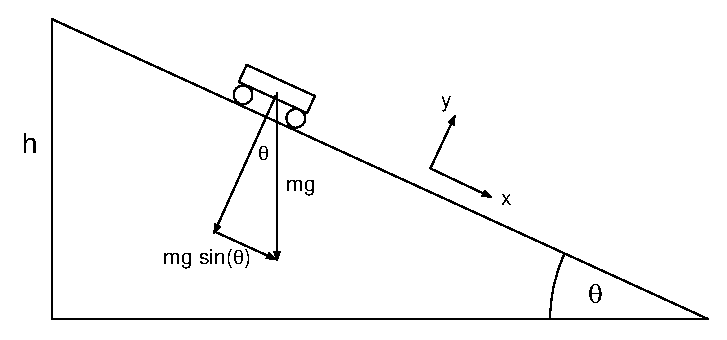
\includegraphics[width=3in]{incline-2}}
  \caption{The free body diagram of the cart moving down an incline
    plane with height $h$ and angle $\theta$. }
  \label{fig:cartInclineFBG}
\end{figure}


\begin{assignment}
  \textbf{Part a}.  Find the acceleration due to gravity, $g$, along
  with its uncertainty from an experiment using a simple pendulum.
  The pendulum has measured length $l~=~.750m~\pm{.005}m$ and a period
  $T~=~1.8~sec~\pm{.2}~sec$.  Since the period of a pendulum is
  ~$T~=~ 2\pi\sqrt{\frac{l}{g}}$, then $g$ is
  \begin{eqnarray}
    g & = & 4{\pi^2}l/T^2.
  \end{eqnarray}
\end{assignment}


\if y\solutions

\textbf{Solution:}

Our best calculation for the acceleration due to gravity is
\begin{eqnarray*}
  g & \approx & (4)({\pi^2})(.75)/({1.75^2}), \\
    & \approx & 9.14 ~ \mathrm{m/sec}^2.
\end{eqnarray*}

And the uncertainty is
\begin{eqnarray*}
\triangle{g} & \approx & \sqrt{
  \left(\frac{df}{dl}\triangle{l}\right)^2 + 
  \left(\frac{df}{dT}\triangle{T}\right)^2}, \\
& = & \sqrt{
  \left(\frac{4\pi^2}{T^2}.005\right)^2 + 
  \left(\frac{-8\pi^2(.75)}{T^3}.2\right)^2}, \\
& \approx & 2.03 ~ \mathrm{m/sec}^2.
\end{eqnarray*}
So the final answer is $g=9~\pm~2 \mathrm{m/sec}^2$. The uncertainty is
relatively large for the value found, mostly because the uncertainty
for the measured period of the pendulum was so high.  

\fi

\textbf{Part b}.  Calculate $g$ again, along with its uncertainty, if
the length of the pendulum is $l=9.70m\pm .05$m, and the new period
is $T~=~6.3~\mathrm{sec}\pm .2$~sec. (Answer: $g=9.6\pm .6\mathrm{m/sec}^2$.)

\textbf{Part c}.  Why did the uncertainty in Part b decrease when the
uncertainty in determining the length of the pendulum increased?  

\if y\solutions

\textbf{Solution:}

The uncertainty with respect to the measurement of $l$ is proportional
to $\frac{1}{T^2}$, and the uncertainty with respect to the
measurement of $T$ is proportional to $\frac{1}{T^3}$.  The period in
the first part is much smaller than in the second part, and the
uncertainty is much greater.

\fi

\begin{assignment}
  Consider a cart of mass $m$ rolling down a frictionless incline of
  height $h$ at an angle of $\theta$, as is shown in Figure
  \ref{fig:cartIncline}.  The height of the incline is measured as
  $ h~=~1.90m~\pm~.01m$ and the angle of the incline is measured as
  $\theta~=~.470~rad ~\pm~.005 $.  Find the time, $t$, it takes for the cart
  starting at rest to reach the bottom of the
  incline, along with the appropriate uncertainty, $\triangle{t}$. \\
  (Hint: If the length of the incline is $l$, then use the equations
  ~$l~=~\frac{h}{\sin(\theta)}$ ~and~~$l~=~\frac{1}{2}g\sin(\theta) t^2$ to
  solve for $t$.)
\end{assignment}

\if y\solutions

\textbf{Solution:}

The terms are related by the relationship
\begin{eqnarray*}
\frac{h}{\sin\theta}~=~\frac{1}{2}~g\sin(\theta) t^2.
\end{eqnarray*}
Solving for the time gives
\begin{eqnarray*}
  t & = & f(h,\theta), \\
  & = & \sqrt{\frac{2h}{g}}\left(\frac{1}{|\sin(\theta)|}\right).
\end{eqnarray*}
The corresponding uncertainty is
\begin{eqnarray*}
  \triangle t & = & \sqrt{
    \left(\frac{\partial f}{\partial h} \triangle h \right)^2 +
    \left(\frac{\partial f}{\partial \theta} \triangle \theta \right)^2 }.
\end{eqnarray*}
In this situation the angle $\theta$ is between 0 and $\frac{\pi}{2}$
so  
\begin{eqnarray*}
  |\sin(\theta)| & = & \sin(\theta).
\end{eqnarray*}
The best estimate for the time is 
\begin{eqnarray*}
  t & = & \left(\sqrt{\frac{2\cdot 1.90}{9.8}}\right)
  \frac{1}{\sin(.470)}, \\
  & \approx & 1.37~sec.
\end{eqnarray*}
The partial derivatives are the following: 
\begin{eqnarray*}
\frac{\partial f}{\partial h} & = & 
\left(\frac{1}{2\sin(\theta)}\right)\left(\sqrt{\frac{2}{gh}}\right)
~ \approx ~ 
\left(\frac{1}{2\sin(0.47)}\right)\left(\sqrt{\frac{2}{9.8\cdot 1.90}}\right)
~ \approx ~ 0.36, \\
\frac{\partial f}{\partial \theta} & = &
-\sqrt{\frac{2h}{g}}\left(\frac{\cos(\theta)}{\sin^2(\theta)}\right)
~ \approx ~ 
-\sqrt{\frac{2\cdot 1.90}{9.8}}\left(\frac{\cos(0.470)}{(\sin(0.470))^2}\right)
~ \approx ~ -2.71.\\
\end{eqnarray*}
The uncertainty can now be approximated by
\begin{eqnarray*}
\triangle{f} & = & \sqrt{
  \left(\frac{\partial f}{\partial h} \triangle{h} \right)^2 +
  \left(\frac{\partial f}{\partial \theta} \triangle{\theta}\right)^2}
~=~.014sec.
\end{eqnarray*}
The estimate for the time is $t~=~1.37sec~\pm~.01sec$.

\fi

\section{Data}
\label{sect:data}

Once a set of observations are conducted and a number of measurements
are made the question is how to analyze the numbers.  First, there are
different kinds of data:
\begin{description}
\item[Categorical Data] Data that consists of discrete groups or
  types. (Ex: polls where people pick one of several options result in
  categorical data.)
\item[Quantitative Data] Data made up of numerical values in which
  arithmetic operations such as adding and multiplying makes sense.
\end{description}

Most of the data collected in a physics laboratory is quantitative
data.  It makes sense to perform algebraic manipulations.  A recurring
example made up of quantitative data is used. The data set is from a
number of measurements that Henry Cavendish observed in
1798\cite{mooreMccabe}.  Cavendish's goal was to measure the density
of the earth, and his numbers are in terms of the ratio of the density
of the earth divided by the density of water. Cavendish's data is
given in Table \ref{table:cavendish}.


\begin{table}[ht]
  \centering
  \begin{tabular}{rrrrrrr}
    5.50 & 5.61 & 4.88 & 5.07 & 5.26 & 5.55 & 5.36 \\
    5.29 & 5.58 & 5.65 & 5.57 & 5.53 & 5.62 & 5.29 \\
    5.44 & 5.34 & 5.79 & 5.10 & 5.27 & 5.39 & 5.42 \\
    5.47 & 5.63 & 5.34 & 5.46 & 5.30 & 5.75 & 5.68 \\
    5.85    \\
  \end{tabular}
  \caption{Henry Cavendish's measurements of the ratio of the density of earth and the density of water.}
  \label{table:cavendish}
\end{table}

One of the first things you should notice when looking at the numbers
Cavendish generated is that they are not all the same. Each time
Cavendish made a measurement a small error was made.  The question
that arises is how to make sense out of all of these different
numbers.

The first step is to explore how to examine and summarize the data.
The two ways are to generate \textit{graphical} and \textit{numerical}
views of the data.

\subsection{Defining the Terms}

There are many different ways that numbers can be generated, and great
care is required about how to communicate findings. The ways that
studies are conducted can be broken down into two broad categories.

\begin{definition}
  In an \textbf{observational study} a set of observations on
  individuals is made. The variables of interest are measured with the
  intent to avoid influencing the responses.
\end{definition}

\begin{definition}
  In an \textbf{experiment} deliberate treatments are imposed to
  varying degrees with measurements of predetermined responses.
\end{definition}

In this course ``experiments'' are the principle way to generate data
and the focus is to use methods that provide good evidence for
causation. It is important to note that an experiment can only
identify association between two variables and not causation.  A good
experiment, however, can provide strong circumstantial evidence for
causation or at least isolate related variables to the smallest degree
possible.

When an experiment is conducted a number of observations are made of a
physical system. For each observation a number of measurements are
made based on the observation. It is important to note that the
process of observing a physical system influences the system and will
impact the variables that are being measured. At the same time errors
are \textbf{always} made when making a measurement. It is not possible
to make an exact measurement. 

Any time a measurement is made based on an observation there will be
some error. The error can be minimized through good experimental
practices, but it will always be present. Errors are always present
requiring the use of careful statistical techniques.

\subsection{Graphical Views of Data}

Graphical views of data is the first topic examined, and stem/leaf
plots and histograms are the first topic. In a stem plot the data is
first put in numerical order and then the numbers are grouped into
discrete sets or ``bins.'' The bins are ordered in a vertical list and
then each number is written across rows by which bin it falls in.

Using the data collected by Cavendish, see Table
\ref{table:cavendish}, The numbers are ordered from smallest
to largest: \\
\begin{center}
\begin{tabular}{rrrrrrrr}
4.88 & 5.07 & 5.10 & 5.26 & 5.27 & 5.29 & 5.29 & 5.30 \\
5.34 & 5.34 & 5.36 & 5.39 & 5.42 & 5.44 & 5.46 & 5.47 \\
5.50 & 5.53 & 5.55 & 5.57 & 5.58 & 5.61 & 5.62 & 5.63 \\
5.65 & 5.68 & 5.75 & 5.79 & 5.85
\end{tabular}
\end{center}

A set of bins must be determined. Here the numbers are collected into
those values that fall into the following categories\footnote{The
  choice of bins is somewhat arbitrary. These bins are used because
  the results can be interpreted relatively easily.}:
\begin{eqnarray*}
  \begin{array}{r@{\hspace{1em}\leq\hspace{1em}x\hspace{1em}<\hspace{1em}}l}
    4.8 & 4.9 \\
    4.9 & 5.0 \\
    5.0 & 5.1 \\
    5.1 & 5.2 \\
    5.2 & 5.3 \\
    5.3 & 5.4 \\
    5.4 & 5.5 \\
    5.5 & 5.6 \\
    5.6 & 5.7 \\
    5.7 & 5.8 \\
    5.8 & 5.9
  \end{array}
\end{eqnarray*}
The numbers on the far left of the list are called the ``stems.''
Given one of the numbers from our data set it can be written as a stem
and a leaf. For example, one of the numbers in our data set is 5.58.
The stem for this number is 5.5 and the leaf is the remaining digit,
8.

To create the stem/leaf plot all of the stems are written in a
vertical list. Next to each stem the leaves are written in numerical
order. The stem/leaf plot for Cavendish's data is given in Table
\ref{tab:cavendishStemLeaf}. It is a crude way to order the data, but
it helps reveal some important features about the data.  Cavendish's
numbers range from 4.88 to 5.85.  Most of the numbers are clustered
around 5.4 but many are spread out between 5.2 and 5.6. The
measurement of 4.88 immediately appears to be different from the other
measurements in this particular view.



\begin{table}
  \centering
\begin{verbatim}
  The decimal point is 1 digit(s) to the left of the |

  48 | 8
  49 | 
  50 | 7
  51 | 0
  52 | 6799
  53 | 04469
  54 | 2467
  55 | 03578
  56 | 12358
  57 | 59
  58 | 5
\end{verbatim}
  \caption{The Stem/Leaf plot for Cavendish's approximation of the relative density of the earth. }
  \label{tab:cavendishStemLeaf}
\end{table}


The idea of a stem/leaf plot can be extended to make a graph based on
how many of the measurements fall within each bin. For example, there
are five measurements that fall within the category for numbers
between 5.3 and 5.4. The number of measurements that fall within a
particular bin is called the ``frequency,'' and a graph of the
frequencies for each bin is called an ``histogram.'' The histogram for
Cavendish's data is shown in Figure \ref{fig:cavHist}.

\begin{figure}[tb]
  \centerline{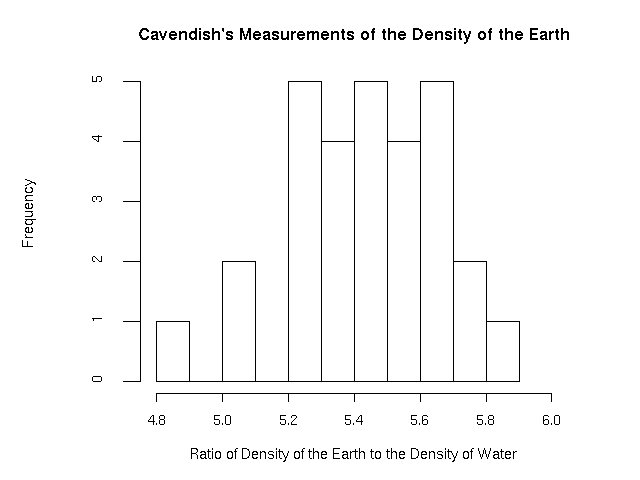
\includegraphics[height=4in]{cavHist}} %,angle=270
  \caption{Histogram of Cavendish's Data}
  \label{fig:cavHist}
\end{figure}

Again, the histogram in Figure \ref{fig:cavHist} demonstrate that the
measurements appear to be centered around 5.4 and equally distributed
between 5.2 and 5.6. The numbers appear to be slightly skewed and a
little more spread out for the lower numbers than the higher numbers.

\begin{assignment}
  Make a stem/leaf plot of the following numbers:
  \begin{center}
    \begin{tabular}{rrrrrr}
      17 & 18 & 9 & 41 & 46 & 16 \\
      34 & 39 & 9 & 9  & 14 & 12 \\
      19 & 8      
    \end{tabular}
  \end{center}
  Use a bin size of 10, that is use the intervals, 0-9, 10-19, 20-29,
  30-39, and 40-49. In this situation the number 8 can be thought of
  as 08, so its stem is 0 and leaf is 8.
\end{assignment}

\if y\solutions

\textbf{Solution:}

First, the numbers are written in order,
\begin{verbatim}
08  09  09  09 12 14 16 17 18 19 34 39 41 46.
\end{verbatim}

%\samepage
Now the stem/leaf plot can be determined:
\begin{verbatim}
  The decimal point is 1 digit(s) to the right of the |

  0 | 8999
  1 | 246789
  2 | 
  3 | 49
  4 | 16
\end{verbatim}
%\pagebreak[0]

\fi

\begin{assignment}
  Make a stem/leaf plot of the following numbers:
  \begin{center}
    \begin{tabular}{rrrrrr}
       1.5 & 7.0 & 0.6 & 4.5 & 3.7 & 5.7 \\
       8.0 & 1.6 & 3.8 & 2.7 & 2.0 & 7.1
    \end{tabular}
  \end{center}
  Use a bin size of 1.
\end{assignment}

\if y\solutions

\textbf{Solution:}

First, the numbers are written in order,
\begin{verbatim}
0.6 1.5 1.6 2.0 2.7 3.7 3.8 4.5 5.7 7.0 7.1 8.0
\end{verbatim}

%\samepage
Now the stem/leaf plot can be determined:
\begin{verbatim}
  The decimal point is at the |

  0 | 6
  1 | 56
  2 | 07
  3 | 78
  4 | 5
  5 | 7
  6 |
  7 | 01
  8 | 0

\end{verbatim}
%\pagebreak[0]

\fi

\begin{assignment}
  Draw a sketch of a histogram for the following numbers:
  \begin{center}
    \begin{tabular}{rrrrrr}
      17 & 18 & 9 & 41 & 46 & 16 \\
      34 & 39 & 9 & 9  & 14 & 12 \\
      19 & 8      
    \end{tabular}
  \end{center}
  Use a bin size of 10, that is use the intervals, 0-9, 10-19, 20-29,
  30-39, and 40-49.
\end{assignment}

\if y\solutions
\textbf{Solution:} 

\centerline{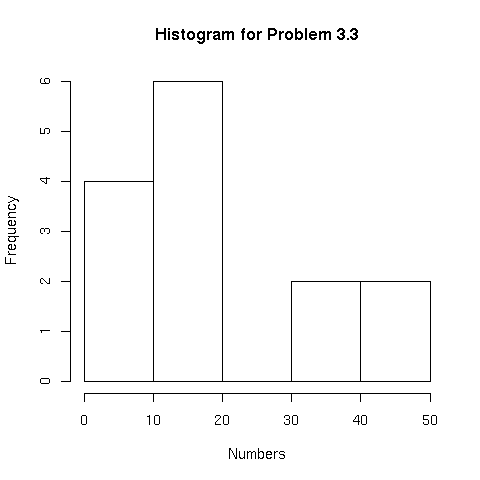
\includegraphics[width=3.5in]{prob33}}
\fi

\begin{assignment}
  Make a stem/leaf plot of the following numbers:
  \begin{center}
    \begin{tabular}{rrrrrr}
       1.5 & 7.0 & 0.6 & 4.5 & 3.7 & 5.7 \\
       8.0 & 1.6 & 3.8 & 2.7 & 2.0 & 7.1
    \end{tabular}
  \end{center}
  Use a bin size of 2.
\end{assignment}

\if y\solutions
\textbf{Solution:} 

\centerline{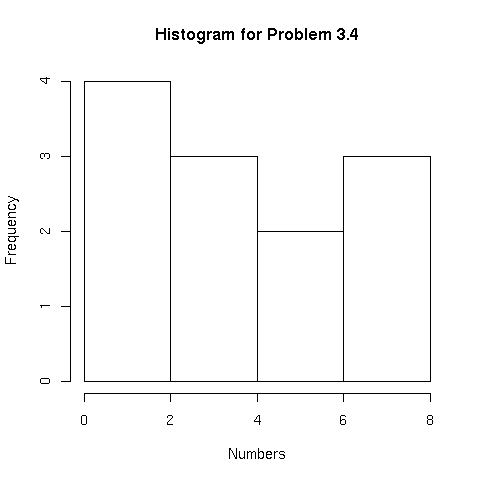
\includegraphics[width=3.5in]{prob34}}
\fi



\subsection{Numerical Views of Data}
\label{subsect:numericalDescription}

In looking at the two graphical views of Cavendish's data the set of
data appears to have two important properties, a \textit{center} and
\textit{spread}. These terms are descriptive but not precise.  Some
definitions are necessary that will help make comparisons and quantify
what is meant by \textit{center} and \textit{spread}.  Unfortunately,
there are multiple ways to measure these things so it is still not
entirely precise.

The first thing that examined is the \textit{center} of the data.
There are three ways to determine the \textit{center}. In the
vernacular many people call this the \textit{average}.  Unfortunately,
the word \textit{average} is commonly used but does not have a
specific definition, and some nefarious people can take advantage of
this\footnote{This can be quite frustrating when reading news reports
  in which knowledgeable people can manipulate the way information is
  perceived.}.  Three different definitions are used to refer to the
\textit{center} of data.



\begin{definition}
  The \textbf{mode} of a set of numbers is the bin that has the
  highest frequency. If the greatest frequency occurs in a number of
  bins then the data is said to be ``multi-modal'' and all of the
  modes are reported. Note that the specification of the mode depends
  on a set of bins of predetermined width that have been defined.
\end{definition}


\begin{definition}
  The \textbf{median} is the number where half of the measurements are
  above it and the other half are below it.
\end{definition}

\begin{definition}
  The \textbf{sample mean} of a set of numbers,
  \begin{eqnarray}
    \label{eqn:sampleObservations}
    x_1,~x_2,~x_3,\ldots,x_n,
  \end{eqnarray}
  is defined to be
  \begin{eqnarray}
    \label{eqn:sampleMean}
    \bar{x} & = & \frac{1}{n} \lp x_1 + x_2 + x_3 + \cdots + x_n \rp, \\
    & = & \frac{1}{n} \sum^n_{k=1} x_k. \nonumber
  \end{eqnarray}
  This is the number that minimizes the sample variance which will be
  defined later. The sample mean is also the number that many people
  \textbf{think} is the ``average'' of a set of numbers, but this is
  not necessarily the case.
\end{definition}

A question that comes up is which method to approximate the center of
the data should be used. The answer is that all of them should be
used. Each measure of the center gives a slightly different view of
the center of the data, and each of them should be used to help
provide a better understanding of a data set.

The different measures for the \textit{center} of Cavendish's data are
the following:
\begin{itemize}
\item If the bins are broken up into widths of .1 just as in the
  previous example, then the data is multi-modal with modes of
  5.2-5.3, 5.4-5.5, and 5.6-5.7.
\item The median is 5.46.
\item The mean is approximately 5.45.
\end{itemize}
Note that in this case the modes, the median, and the mean are all
clustered around one another. There is little ``bias.'' That is the
data is evenly distributed around the different measures of the
\textit{center}.


The spread of the data can be specified in one of two ways. The first
way to measure the spread is to provide the \textit{five number
  summary}. The five number summary consists of reporting the minimum
measurement, the maximum measurement, the median, and the first and
third quartiles. The first quartile is found by taking all of the
numbers that are less than the median and finding the median of that
set of numbers. The third quartile is found by taking all of the
measurements greater than the median and finding the median of that
set of numbers.

These numbers can be found relatively easily using a stem/leaf plot.
For example, the stem/leaf plot in Table \ref{tab:cavendishStemLeaf}
can be used to find the five number summary for Cavendish's
measurements.  The five number summary for Cavendish's measurements
are the following:
\begin{verbatim}
   Min. 1st Qu.  Median  3rd Qu.    Max. 
  4.880   5.300   5.460    5.610   5.850 
\end{verbatim}
By looking at the differences in the minimum
and the first quartile, the first quartile and the median, the median
and the third quartile, and the third quartile and the maximum you can
get an idea of how spread out the numbers are. Again, the numbers are
relatively evenly spread out but appear to be slightly skewed so that
the measurements are more spread out on the low end.

The five point summary can be viewed graphically using a \textit{box
  plot}. A box plot displays the five points as follows:
\begin{itemize}
\item A box shows the first and third quartiles.
\item A line in the box shows the median.
\item Lines extend from the box to the maximum and the minimum.
\end{itemize}
The box plot for Cavendish's data is shown in Figure
\ref{fig:cavBoxPlot}. You can see graphically that it is relatively
evenly distributed but more spread out amongst the low numbers.  (Note
that the mean is generally not indicated in a box plot.)

\begin{figure}[tb]
  \centerline{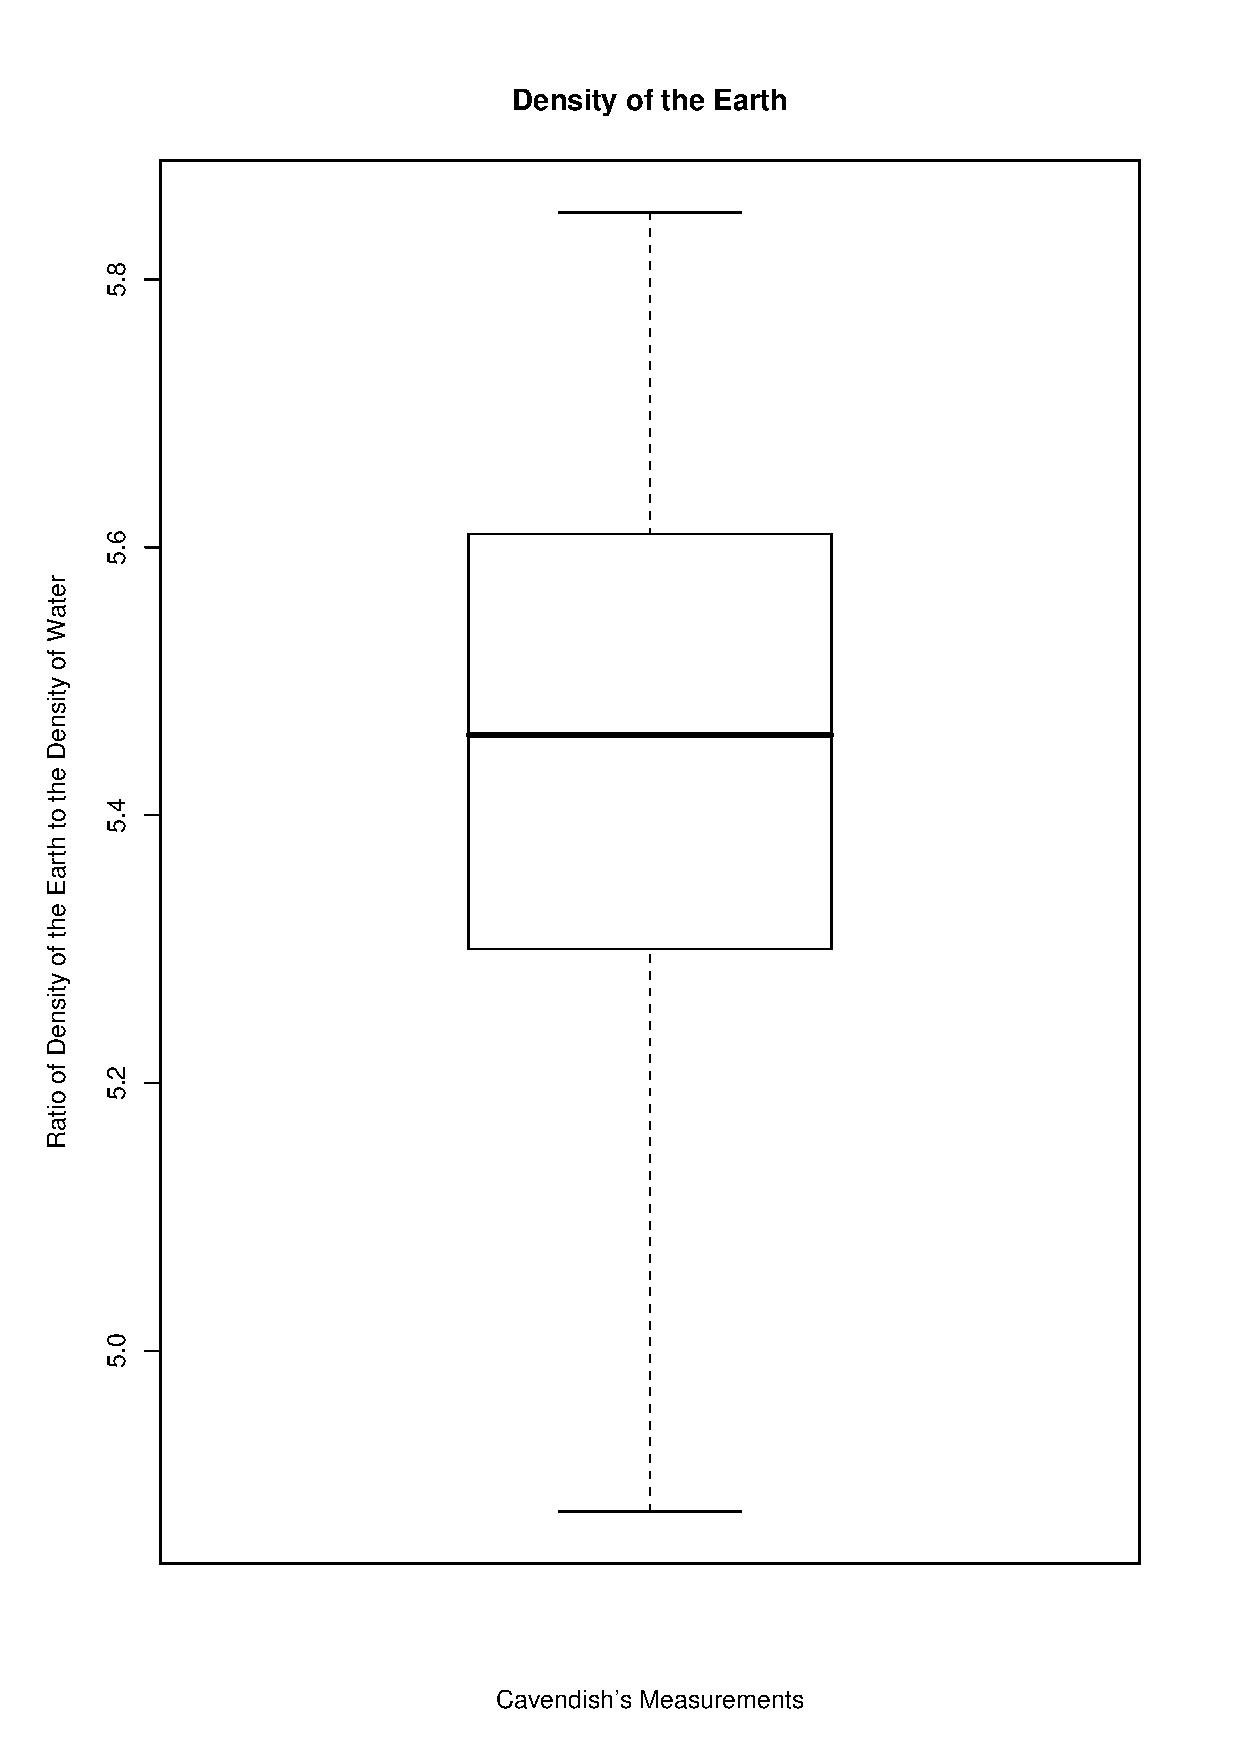
\includegraphics[height=3in]{cavBoxPlot}}
  \caption{Box plot of Cavendish's data.}
  \label{fig:cavBoxPlot}
\end{figure}

Another numerical description of the spread of the data is the
\textit{sample variance}. It is a measure of how the data varies
around the sample mean. This is a circular argument since the sample
mean minimizes the variance, and the two numbers are very closely
linked.  At first it does not seem intuitive to link the two ideas of
``center'' and ``spread'' so closely. Unfortunately, when working with
data it can be difficult to separate the two ideas because they are
closely linked. For example, when discussing the spread of a set of
data you must specify which point the data varies around. At the same
time the amount of trust we can place in a measurement of the center
depends on the spread of the data, an idea that is examined in section
\ref{section:confidenceIntervals}.

\begin{definition}
  The \textbf{sample variance} of a set of numbers,
  \begin{eqnarray*}
    x_1,~x_2,~x_3,\ldots,x_n,
  \end{eqnarray*}
  which have a mean, $\bar{x}$, is
  \begin{eqnarray}
    \label{eqn:sampleVariance}
    s^2_{\rm x} & = & \frac{1}{n-1} \sum^n_{k=1} \lp x_k - \bar{x} \rp^2.
  \end{eqnarray}
\end{definition}

\begin{definition}
  The \textbf{sample standard deviation} is the square root of the
  sample variance,
  \begin{eqnarray}
    \label{eqn:sampleStandardDeviation}
    s_{\rm x} & = & \sqrt{s^2_{\rm x}}.
  \end{eqnarray}
\end{definition}

The measurements made by Cavendish have a mean of approximately 5.45,
a sample variance of approximately  0.049, and a sample standard
deviation of approximately .22.

\begin{assignment}
  Find the five point summary and draw a box plot of the following numbers:
  \begin{center}
    \begin{tabular}{rrrrrr}
      17 & 18 & 9 & 41 & 46 & 16 \\
      34 & 39 & 9 & 9  & 14 & 12 \\
      19 & 8      
    \end{tabular}
  \end{center}

\end{assignment}

\if y\solutions

\textbf{Solution:}

The five point summary is the following:
\begin{verbatim}
   Min. 1st Qu.  Median    Mean 3rd Qu.    Max. 
   8.00    9.75   16.50   20.79   30.25   46.00 
\end{verbatim}

\centerline{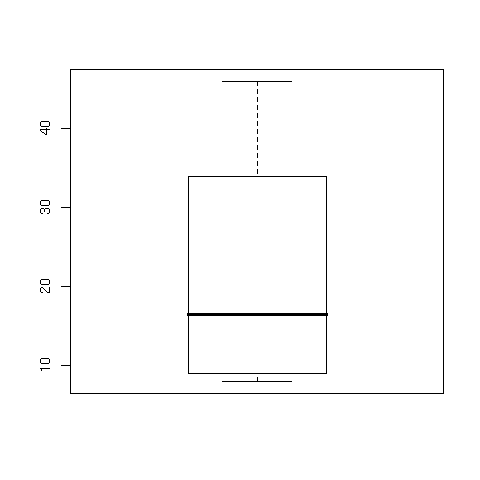
\includegraphics[width=3.5in]{prob35}}

Approximations for the mean, variance, and standard deviations are the
following:
\begin{eqnarray*}
  \bar{x}    & \approx & 20.79 \\
  \sigma^2_x & \approx & 177.10 \\
  \sigma_x   & \approx & 13.31
\end{eqnarray*}

\fi

\begin{assignment}
  Find the five point summary and draw a box plot of the following numbers:
  \begin{center}
    \begin{tabular}{rrrrrr}
       1.5 & 7.0 & 0.6 & 4.5 & 3.7 & 5.7 \\
       8.0 & 1.6 & 3.8 & 2.7 & 2.0 & 7.1
    \end{tabular}
  \end{center}
  Also, find the mean, variance and standard deviation of the numbers.
\end{assignment}

\if y\solutions

\textbf{Solution:}

The five point summary is the following:
\begin{verbatim}
   Min. 1st Qu.  Median    Mean 3rd Qu.    Max. 
  0.600   1.900   3.750   4.017   6.025   8.000 
\end{verbatim}

\centerline{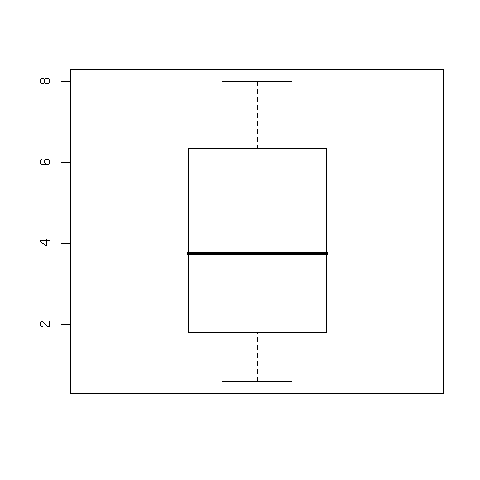
\includegraphics[width=3.5in]{prob36}}

Approximations for the mean, variance, and standard deviations are the
following:
\begin{eqnarray*}
  \bar{x}    & \approx & 4.02  \\
  \sigma^2_x & \approx & 6.10  \\
  \sigma_x   & \approx & 2.47
\end{eqnarray*}


\fi




\begin{assignment}
  Show that the value of $\bar{x}$ given in Equation
  (\ref{eqn:sampleMean}) is the value of $\bar{x}$ that minimizes the
  sample variance given in Equation (\ref{eqn:sampleVariance}). (Hint:
  treat Equation (\ref{eqn:sampleVariance}) as a function of $\bar{x}$
  and then approach this problem as a regular optimization problem.)
\end{assignment}

\if y\solutions

\textbf{Solution:}

From Equation (\ref{eqn:sampleVariance}), the sample variance is
defined by
  \begin{eqnarray}
    s^2_{\rm x} & = & \frac{1}{n-1} \sum^n_{k=1} \lp x_k - \bar{x} \rp^2.
  \end{eqnarray}
To find the value of $\bar{x}$ that minimizes the expression the
derivative with respect to $\bar{x}$ is found and set equal to zero,
\begin{eqnarray*}
  0 & = & \frac{d}{d \bar{x}} s^2_{\rm x}, \\
  & = & \frac{d}{d \bar{x}} \lp \frac{1}{n-1} \sum^n_{k=1} \lp x_k - \bar{x} \rp^2 \rp, \\
  & = & \frac{1}{n-1} \sum^n_{k=1} \frac{d}{d \bar{x}} \lp x_k - \bar{x} \rp^2, \\
  & = & \frac{1}{n-1} \sum^n_{k=1} -2 \lp x_k - \bar{x} \rp, \\
  & = & \frac{-2}{n-1} \lp \sum^n_{k=1}  x_k - \sum^n_{k=1} \bar{x} \rp.
\end{eqnarray*}

After multiplying both sides by $\frac{n-1}{2}$ the expression is
\begin{eqnarray*}
  \sum^n_{k=1}  x_k - \sum^n_{k=1} \bar{x} & = & 0.
\end{eqnarray*}
Since $\bar{x}$ is a constant the second sum simplifies to
\begin{eqnarray*}
  \sum^n_{k=1}  x_k - n \, \bar{x} & = & 0.
\end{eqnarray*}
Solving for $\bar{x}$ gives the expression
\begin{eqnarray*}
  \bar{x} & = & \frac{1}{n} \sum^n_{k=1}  x_k.
\end{eqnarray*}

Note that there is only one solution, and the original expression is
quadratic in $\bar{x}$. Since it is positive and quadratic this must
be a minimum.

\fi

\section{Continuous Random Variables}

When making any measurement there is some random variation that must
be considered.  The idea is formalized and defined in terms of
something called a random variable. Some of the definitions that will
help make sense of random phenomena are given and explored. Finally,
the mean and variance is defined when discussing the center and spread
of a random variable.

\subsection{Definition of a Random Variable}

Whenever a measurement is made during an observation there is some
error. That error is different each time a measurement is made. One of
the goals for the experimenter is to design the experiment to make the
errors small enough that the phenomena of interest can be discerned.
This implies that the goal is not to make the error as small as
possible but small enough. There is always a balance between cost,
time, and the overall scientific goals that must be considered.

The experimenter tries to devise a scheme in which the sample mean of
the measurements is close to the true value, and the spread of the
data should be small. To complicate matters, there is a random
component to any measurement. This implies that a measurement is not
necessarily a function. The number it returns is not always the same
for a given configuration of the experiment.

\begin{definition}
  A random variable is a variable that returns a number that is the
  result of some random phenomena.
\end{definition}

An example of a random variable is Cavendish's measurements of the
relative density of the earth. Each time he made a measurement he
found different numbers.

Random variables are not functions, and there are few definite
statements that can be made about them. Because of this a whole
different kind of language is used when discussing random variables.
First, definitions of some of the notation is given.  (Traditionally,
the font used to describe random variables is different so that they
can be set apart, and a roman type is generally used.) A random
variable can be expressed in the following form:
\begin{eqnarray*}
  {\rm X}(\omega) & = & r.
\end{eqnarray*}
In this example ${\rm X}$ is the random variable. The event in which
the measurement is taking place is $\omega$. Note that the input can
be a situation or event and is not necessarily a real number. The
random variable will always return a real number, denoted $r$ in this
example.

In practice a random variable is sampled, and a number of discrete
observations are used to find values returned by the random variable.
The numbers that a random variable returns have a \textit{center} and
a \textit{spread}. In particular, given some number of measurements
(or observations) the mean and standard deviation of a random variable
need to be determined.  This is not a trivial task since an estimate
of the mean and standard deviation based on a relatively small number
of observations is used.

Unfortunately in practice the mean and standard deviation cannot be
determined. Some of the terms and methods need to be defined before the
techniques that are used can be examined. In fact, two terms, the mean
and standard deviation of a random variable, have already been used
without an adequate definition.  The mean and standard deviation of a
random variable are not the same things as the sample mean and sample
standard deviations that have already been defined.

\subsection{Probability Distribution of a Random Variable}

The only kind of random variables examined here are continuous random
variables. That is a random variable that can return any real number
in a given range. These kind of random variables are not intuitive,
and a good deal of insight and examples are skipped by limiting
ourselves. Unfortunately, the necessary time is not available to give
to this important topic.

A formal definition of a continuous random variable is a random
variable in which the probability that it returns any one particular,
single number is zero. Going back to Cavendish's measurements, the
measurements in his experiment are from a continuous random variable.
It is highly unlikely that a single measurement would return a
predetermined number, say 5.37652, and it does not make sense to even
consider this.  However, it does make sense to ask how likely a
measurement will return a number in a predetermined \textit{range}.
The notation for the probability that a random variable, $\rm{X}$, is
between real numbers $a$ and $b$ is
\begin{eqnarray*}
  p(a \leq {\rm X} \leq b).
\end{eqnarray*}
Two definitions can aid in helping us in our analysis of a random
variable.

\begin{definition}
  Let $f(x)$ be a function whose domain is the set of real numbers and
  the range includes the set of nonnegative real numbers. Then $f$ is
  a probability density function (pdf) if
  \begin{eqnarray*}
    \int^\infty_{-\infty} f(x) ~ dx & = & 1.
  \end{eqnarray*}
\end{definition}

\begin{definition}
  An absolutely continuous random variable is a random variable,
  $\rm{X}$ in which a probability density function, $f(x)$, exists and
  \begin{eqnarray*}
    p(a \leq {\rm X} \leq b) & = & \int^b_a f(x) ~ dx.
  \end{eqnarray*}
\end{definition}

\begin{example}
  Suppose that a random variable, ${\rm Y}$, returns a number between
  0 and 10 with an equal probability over any interval.
\end{example}

The probability density function for ${\rm Y}$ is
\begin{eqnarray}
  \label{eqn:unformZeroTen}
  f(y) & = & \left\{
    \begin{array}{r@{\hspace{1em}}l}
      \frac{1}{10} & 0\leq y \leq 10, \\
      0 & \mathrm{otherwise}. 
    \end{array}
    \right.
\end{eqnarray}

The probability that ${\rm Y}$ is between two and five is 
\begin{eqnarray*}
  p( 2 \leq {\rm Y} \leq 5) & = & \int^5_2 \frac{1}{10} ~ dy, \\
  & = & \frac{3}{10}.
\end{eqnarray*}

The probability that ${\rm Y}$ is between 0 and 10 is 
\begin{eqnarray*}
  p( 0 \leq {\rm Y} \leq 10) & = & \int^{10}_0 \frac{1}{10} ~ dy, \\
  & = & 1.
\end{eqnarray*}

\begin{definition}
  A random variable is ``uniformally distributed'' over an interval if
  its probability distribution function is a constant over that
  interval.
\end{definition}

\begin{definition}
  A random variable is ``normally distributed'' with a mean of $\mu$
  and standard deviation of $\sigma$ if its density function is 
  \begin{eqnarray*}
    f(x) & = & \frac{1}{\sigma\sqrt{2\pi}} e^{-(x-\mu)^2/(2\sigma^2)}.
  \end{eqnarray*}
\end{definition}

There are few naturally occurring normally distributed random
variables, but it is still an important probability density function.
The sample mean of a random variable is itself a random variable whose
density function is approximately normal. A plot of the probability
density function for a normally distributed random variable is given
in Figure \ref{fig:normalDist}.


\begin{figure}[tb]
  \centerline{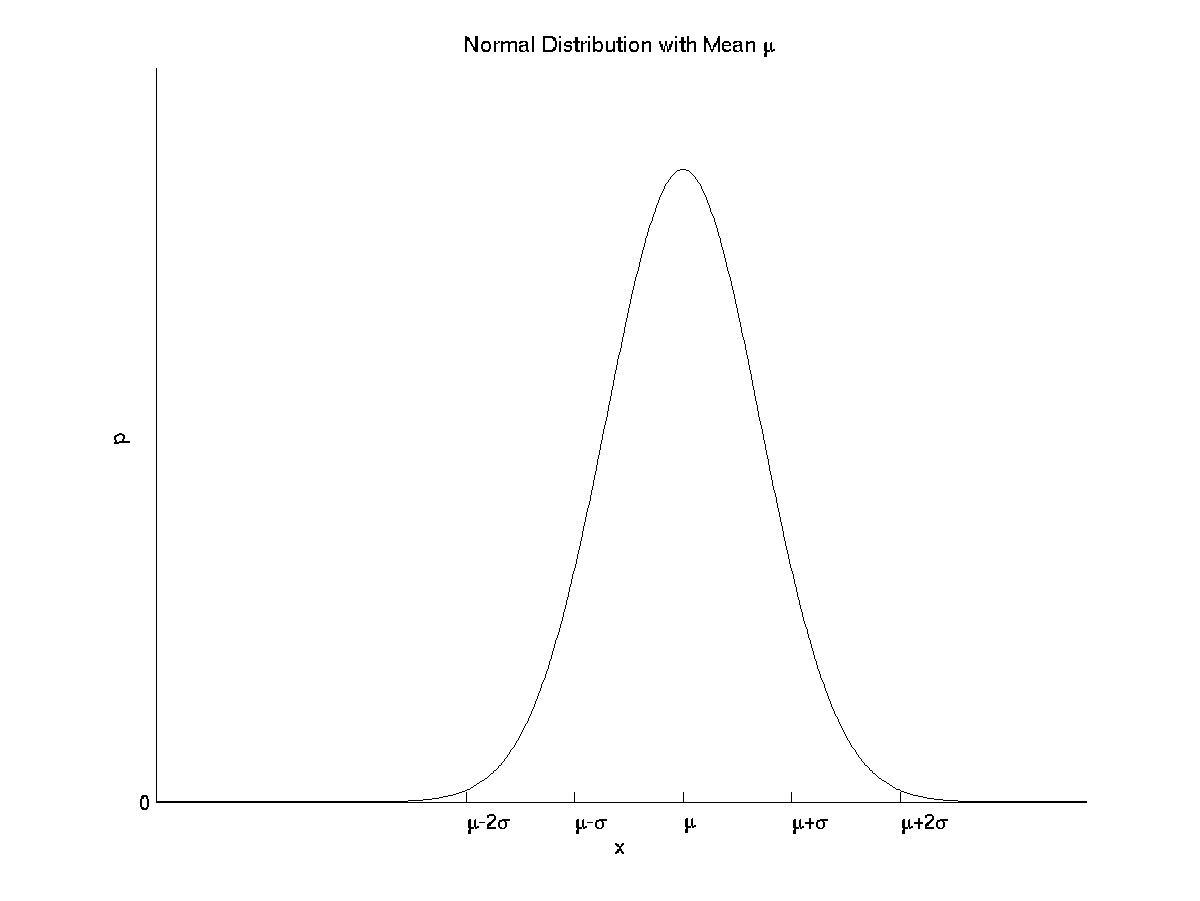
\includegraphics[height=3in]{normal}}
  \caption{Density function for a normally distributed random variable
    with mean $\mu$ and standard deviation $\sigma$.}
  \label{fig:normalDist}
\end{figure}

\begin{assignment}
  A random variable has a probability density function given by
\begin{eqnarray}
  f(x) & = & \left\{
    \begin{array}{r@{\hspace{1em}}l}
      \frac{1}{2}x  & 0\leq x \leq 2, \\
      0 & \mathrm{otherwise}. 
    \end{array}
    \right.
\end{eqnarray}
Find the probability that the random variable returns a number between
0.5 and 1.
\end{assignment}

\if y\solutions

The probability that the random variable returns a number between 0.5
and 1 is 
\begin{eqnarray*}
  \int^1_{0.5} \frac{1}{2} x ~ dx & = & \frac{1}{4} x^2 \bigg|^1_{0.5}, \\
  & = & \frac{1}{4} - \frac{1}{16}, \\
  & = & \frac{3}{16}.
\end{eqnarray*}

\fi


\begin{assignment}
  Show that the function 
  \begin{eqnarray*}
    f(x) & = & \frac{1}{\sigma\sqrt{2\pi}} e^{-(x-\mu)^2/(2\sigma^2)}
  \end{eqnarray*}
  is a probability density function. (Hint: first do a
  $u$-substitution by letting $u=(x-\mu)/\sigma$. Then show that the
  square of the integral,
  \begin{eqnarray*}
    \int^\infty_{-\infty} \frac{1}{\sqrt{2\pi}} e^{-u^2/2} ~ du \, 
    \int^\infty_{-\infty} \frac{1}{\sqrt{2\pi}} e^{-v^2/2} ~  dv & = & 
    \int^\infty_{-\infty} \int^\infty_{-\infty} \frac{1}{2\pi}
    e^{-u^2/2}e^{-v^2/2} ~ du \, dv,
  \end{eqnarray*}
  is one by converting it into polar coordinates.)
\end{assignment}

\if y\solutions

We need to show that 
\begin{eqnarray*}
  \int^\infty_{-\infty} \frac{1}{\sigma\sqrt{2\pi}}
  e^{-(x-\mu)^2/(2\sigma^2)} ~ dx & = & 1.
\end{eqnarray*}
Using a $u$-substitution, $u=(x-\mu)/\sigma$, the integral can be
expressed by
\begin{eqnarray*}
  \int^\infty_{-\infty} \frac{1}{\sqrt{2\pi}} e^{-u^2/2} ~ du & = & 1.
\end{eqnarray*}
Squaring the left hand side gives
\begin{eqnarray*}
  \lp \int^\infty_{-\infty} \frac{1}{\sqrt{2\pi}} e^{-u^2/2} ~ du \rp^2 
  & = & \int^\infty_{-\infty} \frac{1}{\sqrt{2\pi}} e^{-u^2/2} ~ du 
  \int^\infty_{-\infty} \frac{1}{\sqrt{2\pi}} e^{-v^2/2} ~ dv.
\end{eqnarray*}

The new expression can be written as a double integral,
\begin{eqnarray*}
\int^\infty_{u=-\infty} \int^\infty_{v=-\infty} 
    \frac{1}{2\pi} e^{-u^2/2} e^{-v^2/2} ~ dv du & = & 
\int^\infty_{u=-\infty} \int^\infty_{v=-\infty} 
    \frac{1}{2\pi} e^{-(u^2+v^2)/2} ~ dv du.
\end{eqnarray*}
Transforming the integral using polar coordinates yields the expression
\begin{eqnarray*}
\int^\infty_{u=-\infty} \int^\infty_{v=-\infty} 
    \frac{1}{2\pi} e^{-(u^2+v^2)/2} ~ dv du & = & 
\int^\infty_{r=0} \int^{2\pi}_{\theta=0} \frac{1}{2\pi} e^{-r^2/2} r ~ d\theta dr, \\
& = & 
\int^\infty_{r=0}  \frac{2\pi}{2\pi} e^{-r^2/2} r ~ dr, \\
& = & \lim_{R \rightarrow \infty} -e^{R^2/2} + 1, \\
& = & 1.
\end{eqnarray*}


\fi


Another important topic is the analysis of combinations of random
variables, ${\rm X}$ and ${\rm Y}$. Taken together, the probability
that the two random variables are between some set of numbers is
\begin{eqnarray*}
  p( a \leq {\rm X} \leq b,~\mathrm{and}~c \leq {\rm Y} \leq d ).
\end{eqnarray*}
An important idea that is used later is to ask about the
interdependence of two random variables.


\begin{definition}
Two random variables are independent if 
\begin{eqnarray*}
  p( a \leq {\rm X} \leq b,~\mathrm{and}~c \leq {\rm Y} \leq d ) 
  & = & 
  p( a \leq {\rm X} \leq b) \cdot p(c \leq {\rm Y} \leq d ).
\end{eqnarray*}  
\end{definition}

\subsection{Mean and Variance of a Random Variable}

The measure of center and spread of a random variable is similar to
the definition for sampled data but is examined in the context of a
continuous random variable.  A measure of the center is examined
first.  Again, the necessary time is not available to look at these
ideas in the detail and rigor that they deserve and only provide a
cursory glimpse.

\begin{definition}
  If a random variable, ${\rm X}$, is absolutely continuous with
  density function $f$, then the \textbf{expectation} of ${\rm X}$ is
  \begin{eqnarray*}
    E[{\rm X}] & = & \int^\infty_{-\infty} x f(x)~dx.
  \end{eqnarray*}
  (The expectation of a random variable is also called its
  \textbf{mean}.)  The expectation of ${\rm X}$ is sometimes denoted
  in short hand as $\mu_{\rm X}$.
\end{definition}

Note that because $f(x)$ in the equation above is a probability
density function,
\begin{eqnarray*}
  \int^\infty_{-\infty} f(x)~dx & = & 1.
\end{eqnarray*}
As defined the expectation can be written as 
\begin{eqnarray*}
  E[{\rm X}] & = & \frac{\int^\infty_{-\infty} x f(x)~dx}{\int^\infty_{-\infty} f(x)~dx}.
\end{eqnarray*}
If you think of the line as a long thin wire with density $f(x)$ then
the numerator in this expression is the first moment of the wire, and
the denominator is the mass of the wire. The definition of the
expectation is the center of mass for the wire. The expectation is the
point around which the wire will balance.

From the definition of the center the spread of a random variable can
be defined. This definition is similar to the definition of the sample
variance. Because the random variable can return any number an
integral is used rather than a discrete sum, and the squares of the
distances are normalized by their respective probabilities.

\begin{definition}
  If a random variable, ${\rm X}$, is absolutely continuous with
  density function $f$, then the \textbf{variance} of ${\rm X}$ is
  \begin{eqnarray*}
    \mathrm{Var}[{\rm X}] & = & E\left[ ({\rm X}-\mu_{\rm X})^2 \right].
  \end{eqnarray*}
  The variance of ${\rm X}$ is sometimes denoted in short hand as
  $\sigma^2_{\rm X}$.
\end{definition}

\begin{definition}
  The standard deviation of a random variable, ${\rm X}$, is the
  square root of its variance. It is sometimes denoted in short
  hand as $\sigma_{\rm X}$ and
  \begin{eqnarray*}
    \sigma_{\rm X} & = & \sqrt{\sigma_{\rm X}^2}.
  \end{eqnarray*}
\end{definition}

\begin{example}
  What is the mean and standard deviation of a random variable, ${\rm
    X}$, that has a uniform distribution over the interval from zero
  to ten.
\end{example}

The distribution function is the same as the distribution function
given in Equation (\ref{eqn:unformZeroTen}). The mean is
\begin{eqnarray*}
  E[{\rm X}] & = & \int^{10}_0 x \frac{1}{10} ~ dx, \\
  & = & \frac{1}{20} x^2 \bigg|^{10}_0, \\
  & = & \frac{100}{20}, \\
  & = & 5.
\end{eqnarray*}

The standard deviation is the square root of the variance, and first
the variance is found,
\begin{eqnarray*}
  \mathrm{Var}[{\rm X}] & = & 
  \int^{10}_0 \lp x-5 \rp^2 \frac{1}{10} ~ dx, \\
  & = & \frac{(x-5)^3}{30} \bigg|^{10}_0, \\
  & = & \frac{5^3}{30} - \frac{(-5)^3}{30}, \\
  & = & \frac{125}{15}, \\
  & = & \frac{25}{3}.
\end{eqnarray*}
The standard deviation is 
\begin{eqnarray*}
  \sigma_{\rm X} & = & \frac{5}{\sqrt{3}}.
\end{eqnarray*}



As stated previously, the sum of random variables is important. A
comprehensive examination requires the definition of \textit{joint
  probability distributions} and is beyond the scope of this
treatment. Instead some of the basic ideas are given. In the case of
the sum of two random variables, ${\rm X}+{\rm Y}$, the mean is
\begin{eqnarray*}
  E[{\rm X}+{\rm Y}] & = & E[{\rm X}] + E[{\rm Y}], \\
  & = & \mu_{\rm X} + \mu_{\rm Y}.
\end{eqnarray*}
Also, if $r$ is a real number then
\begin{eqnarray*}
  E[r{\rm X}] & = & r E[{\rm X}].
\end{eqnarray*}

Unfortunately calculating the variance can be a little more tricky,
\begin{eqnarray*}
  \mathrm{Var}[{\rm X} + {\rm Y}] & = & 
  E[({\rm X}+{\rm Y}) - (\mu_{\rm X}+\mu_{\rm Y}))^2] \\
  & = & E[({\rm X}-\mu_{\rm X})^2 -
          2({\rm X}-\mu_{\rm X})({\rm Y}-\mu_{\rm Y})+
          ({\rm Y}-\mu_{\rm Y})^2] \\
  & = & E[({\rm X}-\mu_{\rm X})^2] -
        2E[({\rm X}-\mu_{\rm X})({\rm Y}-\mu_{\rm Y})]+
        E[({\rm Y}-\mu_{\rm Y})^2].
\end{eqnarray*}
The middle term, $E[({\rm X}-\mu_{\rm X})({\rm Y}-\mu_{\rm Y})]$, is
called the covariance of the two random variables. If the two random
variables are independent then the covariance is zero. A special case
of the sum of two independent random variables yields the following
result:
\begin{eqnarray}
  \label{eqn:varianceSumTwo}
  \mathrm{Var}[{\rm X} + {\rm Y}] 
  & = & E[({\rm X}-\mu_{\rm X})^2] + E[({\rm Y}-\mu_{\rm Y})^2], \\
  & = & \mathrm{Var}[{\rm X}] + \mathrm{Var}[{\rm Y}].
                                \nonumber
\end{eqnarray}

Finally, if $r$ is a real number then
\begin{eqnarray}
  \label{eqn:varianceScaled}
  \mathrm{Var}[r{\rm X}] & = & r^2 \mathrm{Var}[{\rm X}],
\end{eqnarray}
which implies that the standard deviation of $r{\rm X}$ is $|r|$ times
the standard deviation of ${\rm X}$.


\begin{assignment}
  Find the mean, variance, and standard deviation of a random variable
  that is uniformly distributed on the interval 0 to 1.
\end{assignment}

\if y\solutions

\textbf{Solution:}

The probability density function is
\begin{eqnarray*}
  f(x) & = & \left\{
    \begin{array}{r@{\hspace{1em}}l}
      1 & 0\leq x \leq 1, \\
      0 & \mathrm{otherwise}. 
    \end{array}
    \right.
\end{eqnarray*}
The mean of the random variable is 
\begin{eqnarray*}
  \bar{x} & = & \int^1_0 x \cdot 1 ~ dx, \\
  & = & \frac{1}{2} x^2 \bigg|^1_0, \\
  & = & \frac{1}{2}.
\end{eqnarray*}
The variance is
\begin{eqnarray*}
  \sigma^2_x & = & \int^1_0 \lp x - \frac{1}{2} \rp^2 ~ dx, \\
  & = & \frac{1}{3} \lp x - \frac{1}{2} \rp^3 \bigg|^1_0, \\
  & = & \frac{1}{3} \lp \frac{1}{2} \rp^2 - 
  \frac{1}{3} \lp -\frac{1}{2} \rp^3, \\
  & = & \frac{1}{6}.
\end{eqnarray*}
The standard deviation is
\begin{eqnarray*}
  \sigma_x & = & \sqrt{\frac{1}{6}}.
\end{eqnarray*}


\fi

\begin{assignment}
  Find the mean, variance and standard deviation of a random variable
  whose probability density function is given by
  \begin{eqnarray*}
    f(x) & = & \left\{
      \begin{array}{l@{\hspace{2em}}r}
        \frac{1}{2} x & 0 \leq x \leq 2, \\
        0 & \mathrm{otherwise.}
      \end{array}
      \right.
  \end{eqnarray*}
\end{assignment}

\if y\solutions

\textbf{Solution:}

The mean of the random variable is 
\begin{eqnarray*}
  \bar{x} & = & \int^2_0 x \cdot \frac{1}{2}x ~ dx, \\
  & = & \frac{1}{6} x^3 \bigg|^2_0, \\
  & = & \frac{4}{3}.
\end{eqnarray*}
The variance is
\begin{eqnarray*}
  \sigma^2_x & = & \int^2_0 \lp x - \frac{4}{3} \rp^2 \frac{1}{2}x ~ dx, \\
  & = & \int^2_0 \lp x^2 - \frac{8}{3} x + \frac{16}{9} \rp \frac{1}{2} x ~ dx, \\
  & = & \int^2_0 \frac{1}{2} x^3 - \frac{4}{3} x^2 + \frac{8}{9} x ~ dx, \\
  & = & \frac{1}{8} x^4 - \frac{4}{9} x^2 + \frac{4}{9} x^3 \bigg|^2_0, \\
  & = & 2 - \frac{16}{9} + \frac{32}{9} \\
  & = & \frac{34}{9}.
\end{eqnarray*}
The standard deviation is
\begin{eqnarray*}
  \sigma_x & = & \frac{\sqrt{34}}{3}.
\end{eqnarray*}


\fi



%\begin{assignment}
%    Show that a normally distributed random variable with density function 
%  \begin{eqnarray*}
%    f(x) & = & \frac{1}{\sigma\sqrt{2\pi}} e^{-(x-\mu)^2/(2\sigma^2)}
%  \end{eqnarray*}
%  has a mean of $\mu$ and a standard deviation of $\sigma$.
%\end{assignment}
%
%\if y\solutions
%
%
%Need solution here.
%
%\fi



\section{Sampling Distributions}

One of the first topics examined is some of the basic, descriptive
statistics used to analyze a set of data that has been observed in an
experiment.  A (very) short detour to discuss some of the underlying
theory is given.  Now some of these ideas are brought together. In
particular, given a set of measurements from observations, Equation
(\ref{eqn:sampleObservations}), the sample mean, Equation
(\ref{eqn:sampleMean}), and the corresponding sample standard
deviation, Equation (\ref{eqn:sampleStandardDeviation}), can all be
determined.

Since each measurement is a random variable, the sample mean is a sum
of random variables, and the sample mean itself is a random variable.
The same result follows for the sample standard deviation for the same
reasons. The consequences of this and the main result is the central
limit theorem which states that the sample mean can be approximated as
a normal distribution and the standard deviation depends on the number
of observations.

\subsection{The Sample Mean as a Random Variable}
\label{subsect:sampleMeanRV}

As discussed in subsection \ref{subsect:numericalDescription}, an
experiment consists of a number of observations, and within each
observation a set of measurements is made. If $n$ observations are
made, and within a given observation, observation $i$, a single
measurement, $x_i$, is found then a sequence of samples is created,
\begin{eqnarray*}
  x_1, ~ x_2, ~ x_3, ~\ldots,~x_n.
\end{eqnarray*}

Each measurement is a particular sample of a quantity of interest and
is a random variable. Some assumptions about the relationships between
these measurements is required. Basically, the assumptions taken
together imply that the measurements are done consistently and the
experiment is well executed:
\begin{itemize}
\item Each measurement is a measurement from a random variable.
\item The mean of each measurement is the same, $E[x_i]=\mu_{\rm X}$.
\item The variance of each measurement is the same and
  $\mathrm{Var}[x_i]=\sigma_{\rm X}^2$. (i.e. the standard deviation of
  each measurement is $\sigma_{\rm X}$.)
\item The measurements are all independent of one another. (i.e. the
  covariance of any two different observations is zero.)
\end{itemize}

From the definition of the sample mean,
\begin{eqnarray*}
  \bar{x} & = & \frac{1}{n} \lp x_1+x_2+x_3+\cdots +x_n \rp,
\end{eqnarray*}
$\bar{x}$ is a random variable because it is the sum of a set of
random variables. An important goal is to determine the relationship
between the sample mean and the quantity that we are trying to
measure. First the mean and variation of the sample mean are
determined.

The expectation of the sample mean is
\begin{eqnarray}
  E[\bar{x}] & = & E\left[\frac{1}{n} \lp x_1+x_2+x_3+\cdots +x_n \rp\right],
  \nonumber \\
   & = & \frac{1}{n} E[x_1+x_2+x_3+\cdots +x_n], \nonumber \\
   & = & \frac{1}{n} \lp E[x_1]+E[x_2]+E[x_3]+\cdots+E[x_n]\rp,
   \nonumber \\
   & = & \frac{1}{n} \nonumber \lp
   \mu_{\rm{x}}+\mu_{\rm{x}}+\mu_{\rm{x}}+\cdots\mu_{\rm{x}}\rp,
   \nonumber \\
   & = & \frac{1}{n} n \mu_{\rm{x}}, \nonumber \\
   & = & \mu_{\rm{x}}. 
   \label{eqn:expectedSampleMean}
\end{eqnarray}
So the expectation of the sample mean is the mean of each individual
measurement. Off hand, this result would seem to indicate that taking
many measurements and then finding the sample mean does not offer an
advantage. After all, the number you should expect to get is the same.
It is not until looking at the variance that the true advantage is
apparent.

The variance of the sample mean is now examined. The result in
Equation (\ref{eqn:varianceScaled}) for scaling a random variable
implies that
\begin{eqnarray*}
  \mathrm{Var}[\bar{x}] & = & 
  \mathrm{Var}\left[\frac{1}{n} \lp x_1+x_2+x_3+\cdots +x_n \rp\right] \\
  & = & \frac{1}{n^2} \mathrm{Var}[x_1+x_2+x_3+\cdots +x_n]
\end{eqnarray*}
Each measurement is assumed to be independent and equation
(\ref{eqn:varianceSumTwo}) implies that
\begin{eqnarray*}
  \mathrm{Var}[\bar{x}] & = & 
  \frac{1}{n^2} \mathrm{Var}\left[ x_1+x_2+x_3+\cdots +x_n \right] \\
  & = & \frac{1}{n^2} 
  \lp \mathrm{Var}[x_1]+\mathrm{Var}[x_2]+\mathrm{Var}[x_3]+\cdots
  +\mathrm{Var}[x_n] \rp.
\end{eqnarray*}
Assuming that the result of each measurement has the same variance
simplifies the result,
\begin{eqnarray}
  \mathrm{Var}[\bar{x}] & = & \frac{1}{n^2} 
  \lp \sigma^2_{\rm X}+\sigma^2_{\rm X}+\sigma^2_{\rm X}+\cdots
  +\sigma^2_{\rm X} \rp, \nonumber \\
  \label{eqn:varSampleMean}
  & = & \frac{1}{n} \sigma^2_{\rm X}.
\end{eqnarray}
The variance in the sample means decreases like $\frac{1}{n}$. For
example, if number of measurements is doubled then the variance is cut
in half.

Once the variance is known the standard deviation of the sample mean
can be found. The standard deviation of a sample mean of $n$ samples
is
\begin{eqnarray}
  \label{eqn:sdSampleMean}
  \sigma_{\bar{x}} & = & \frac{\sigma_{\rm X}}{\sqrt{n}}.
\end{eqnarray}
The variance decreases like one over $n$, and the standard deviation
decreases like one over $\sqrt{n}$.

After taking a number of measurements and finding the sample mean the
expected result is the same as the expected result for any one
measurement. The spread around the mean, however, is reduced.  If you
just take one measurement then the number you get could be over a wide
range. If you take many measurements and find the sample mean then the
spread around the true mean is reduced. You can place greater trust
that your measurement is close to the true mean.



\subsection{The Central Limit Theorem}

The importance of the results in equations
(\ref{eqn:expectedSampleMean}) and (\ref{eqn:varSampleMean}) cannot be
overstated. Together they make it possible to conduct an experimental
examination of a phenomena and establish some level of confidence in
the result. Whenever you conduct an experiment a number of
measurements from a set of observations must be brought together, but
there is always a problem in that you cannot be absolutely sure that
the measurements are close to the true value.

The sample mean is a random variable. The mean of the sample mean is
the same as the mean for a single measurement, and the variance of a
sample mean with $n$ measurements is $\frac{1}{n}$ times the variance
of a single measurement. There is one more result that ties these
ideas together and to make them truly useful, the Central Limit
Theorem.

The proof of the central limit is technical and requires a great deal
of probability and time. The theorem is simply stated here with some
motivation of why it is important. An example is given of how useful
it can be.

\begin{theorem}
  \label{thm:centralLimit}
  (The Central Limit Theorem) Suppose that $x_1$, $x_2$,
  $\ldots$,$x_n$, are a sequence of random variables consistent with
  the conditions given at the beginning of subsection
  \ref{subsect:sampleMeanRV}. Then the sample mean
  \begin{eqnarray*}
    \bar{x} & = & \frac{1}{n} \lp x_1+x_2+\ldots +x_n \rp,
  \end{eqnarray*}
  is close to a normally distributed random variable with mean
  $\mu_{\rm X}$ and standard deviation $\frac{\sigma_{\rm
      X}}{\sqrt{n}}$ for large $n$.
\end{theorem}

The statement is purposely vague. It is not clear what it means to be
``close.'' That is a difficult question because there are many
different ways that something can converge to a particular value. In
this case the convergence is in ``distribution'' which in theory is a
weak way for one thing to get close to another. In practice, however,
the Central Limit Theorem is much more robust than the theory might
indicate.

An example is used to help motivate the idea. A random variable is
examined whose probability distribution function is uniform on the
interval from zero to one. In other words, if you make a single
observation a number between zero and one will be returned with equal
probability. The expected value of this random variable is one half.
The random variable is sampled 200 times, and the resulting histogram
is shown in Figure \ref{fig:centralLimitOne}.  The histogram is
relatively uniform, and the samples are evenly spread out over the
whole range.

In Figures \ref{fig:centralLimitOne} through
\ref{fig:centralLimitSeven} the histograms of the means for different
random samples is shown. In Figure \ref{fig:centralLimitTwo}, 200
trials were run. In each trial two samples, $x_1$ and $x_2$, from the
random variable were observed and the mean, $\frac{1}{2}\left( x_1 +
  x_2 \right)$, calculated for each trial.  The histogram for the
means from the trials is shown in Figure \ref{fig:centralLimitTwo}.

In Figure \ref{fig:centralLimitThree}, 200 trials were run. In each
trial three samples from the random variable were observed and the
mean calculated for each trial. The histogram for the means from the
trials is shown in Figure \ref{fig:centralLimitThree}. In the
subsequent figures, Figures \ref{fig:centralLimitFour} to
\ref{fig:centralLimitSeven}, the sample size in each trial is
increased from four samples to seven samples.

\begin{figure}[htp]
  \centerline{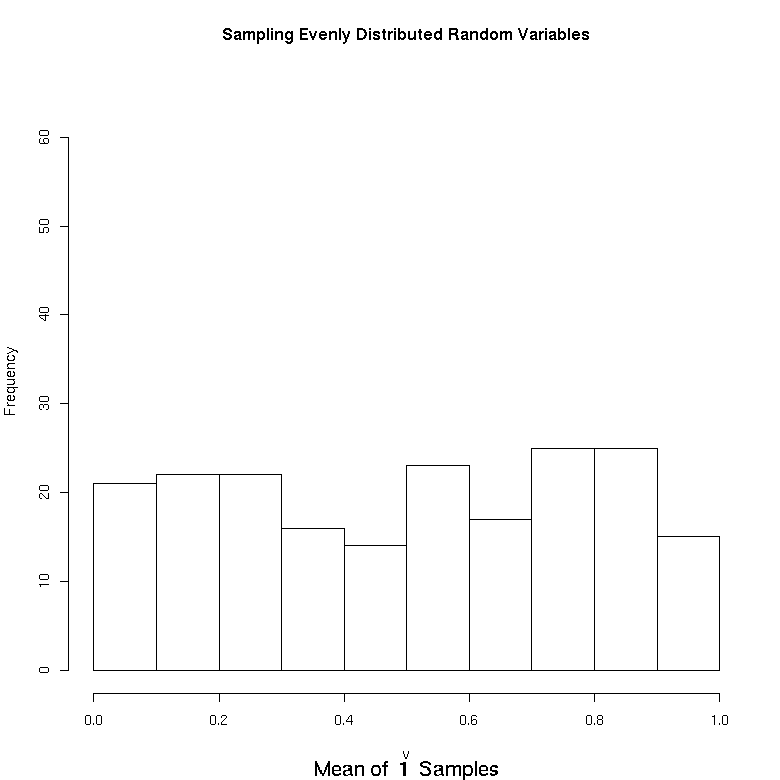
\includegraphics[height=3in]{centralLimit1}}
  \caption{Histogram of 200 random samples of random variable
    uniformly distributed between 0 and 1.}
  \label{fig:centralLimitOne}
\end{figure}

\begin{figure}[htp]
  \centerline{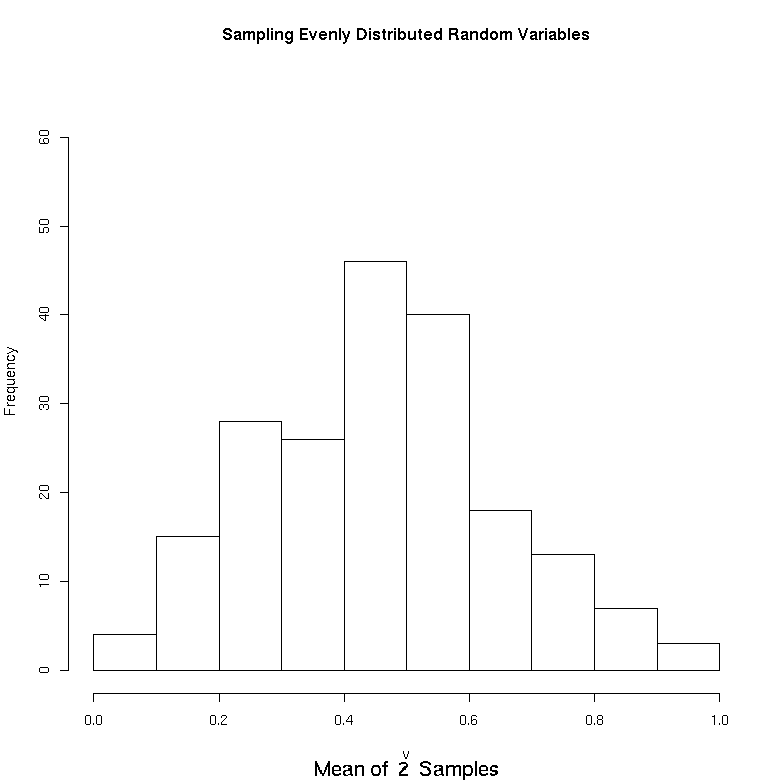
\includegraphics[height=3in]{centralLimit2}}
  \caption{Histogram of 200 trials from a random variable uniformly
    distributed between 0 and 1. Each trial consists of the sample
    mean of 2 samples.}
  \label{fig:centralLimitTwo}
\end{figure}

\begin{figure}[htp]
  \centerline{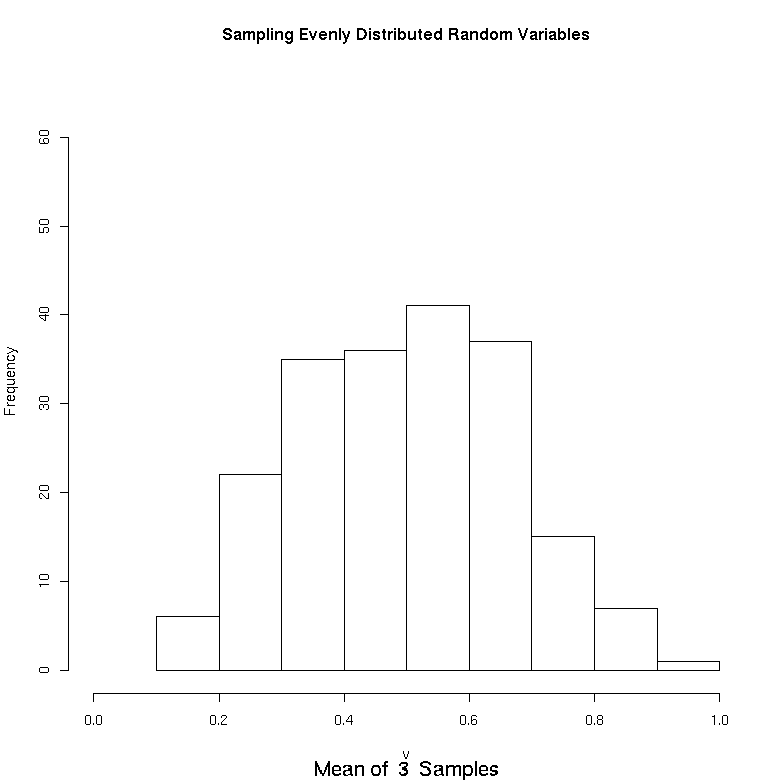
\includegraphics[height=3in]{centralLimit3}}
  \caption{Histogram of 200 trials from a random variable uniformly
    distributed between 0 and 1. Each trial consists of the sample
    mean of 3 samples.}
  \label{fig:centralLimitThree}
\end{figure}

\begin{figure}[htp]
  \centerline{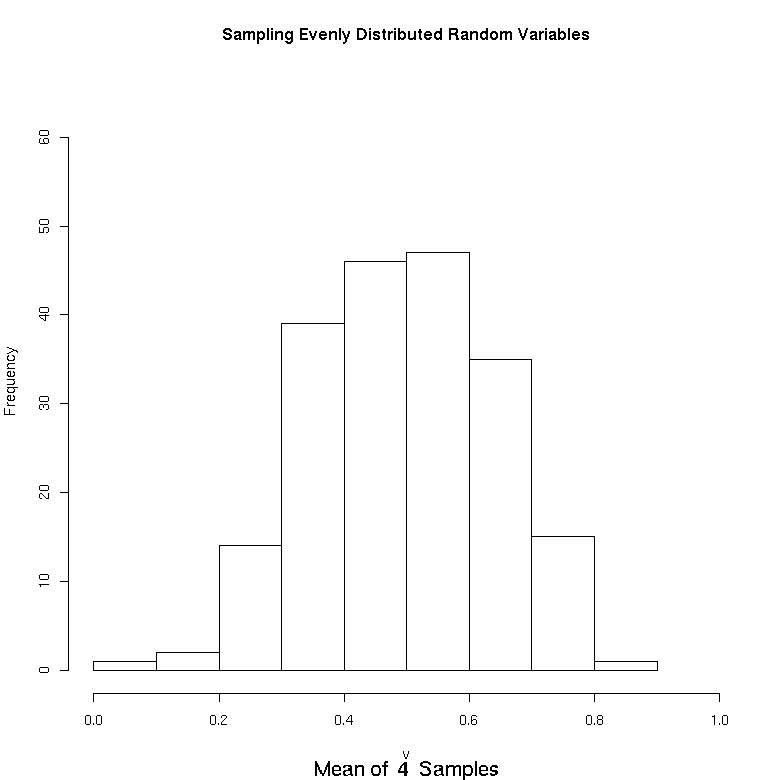
\includegraphics[height=3in]{centralLimit4}}
  \caption{Histogram of 200 trials from a random variable uniformly
    distributed between 0 and 1. Each trial consists of the sample
    mean of 4 samples.}
  \label{fig:centralLimitFour}
\end{figure}


\begin{figure}[htp]
  \centerline{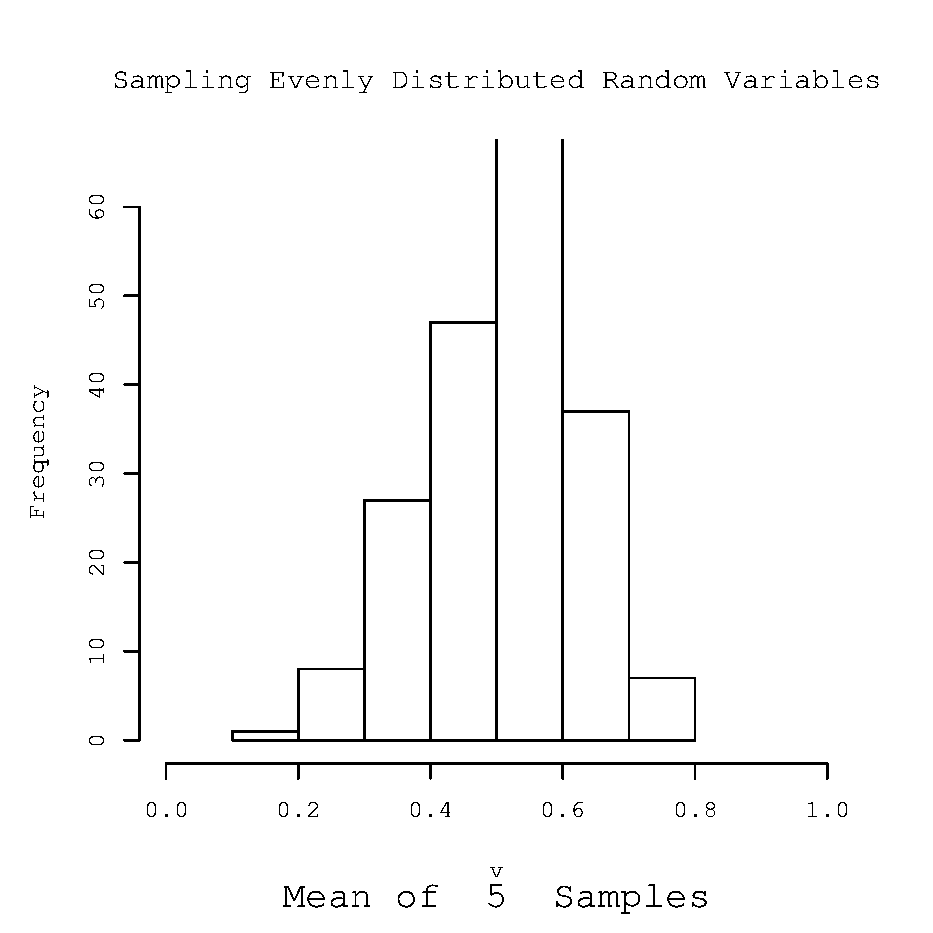
\includegraphics[height=3in]{centralLimit5}}
  \caption{Histogram of 200 trials from a random variable uniformly
    distributed between 0 and 1. Each trial consists of the sample
    mean of 5 samples.}
  \label{fig:centralLimitFive}
\end{figure}

\begin{figure}[htp]
  \centerline{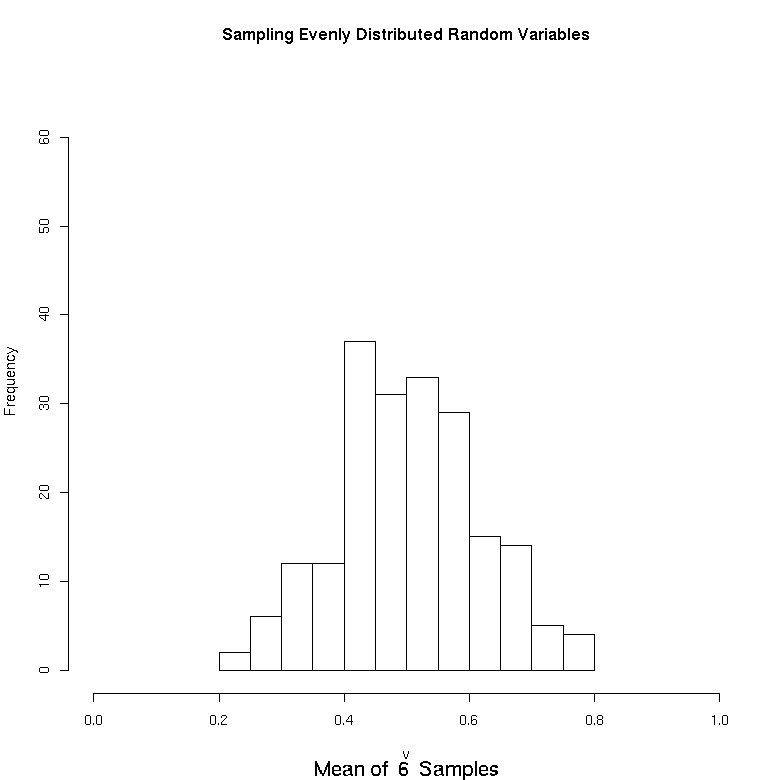
\includegraphics[height=3in]{centralLimit6}}
  \caption{Histogram of 200 trials from a random variable uniformly
    distributed between 0 and 1. Each trial consists of the sample
    mean of 6 samples.}
  \label{fig:centralLimitSix}
\end{figure}

\begin{figure}[htp]
  \centerline{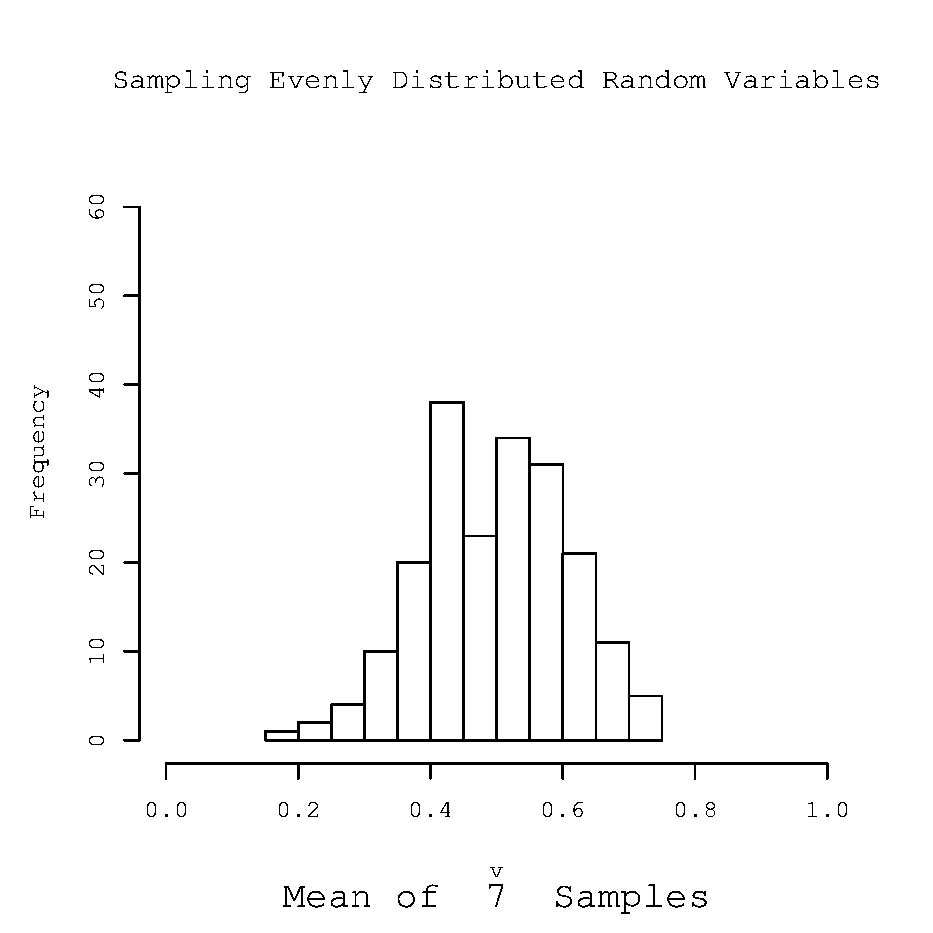
\includegraphics[height=3in]{centralLimit7}}
  \caption{Histogram of 200 trials from a random variable uniformly
    distributed between 0 and 1. Each trial consists of the sample
    mean of 7 samples.}
  \label{fig:centralLimitSeven}
\end{figure}

The histogram in Figure \ref{fig:centralLimitOne} is close to being
uniformly distributed. The histogram in Figure
\ref{fig:centralLimitTwo}, however, is different. The sample
distribution is more closely bunched around the expected value of the
random variable, one half. As the sample size increases in Figures
\ref{fig:centralLimitThree} through \ref{fig:centralLimitSeven} the
sample distribution appears to be more like a normal distribution with
the peak of the distribution near the expected value of the random
variable.


\begin{figure}[htp]
  \centerline{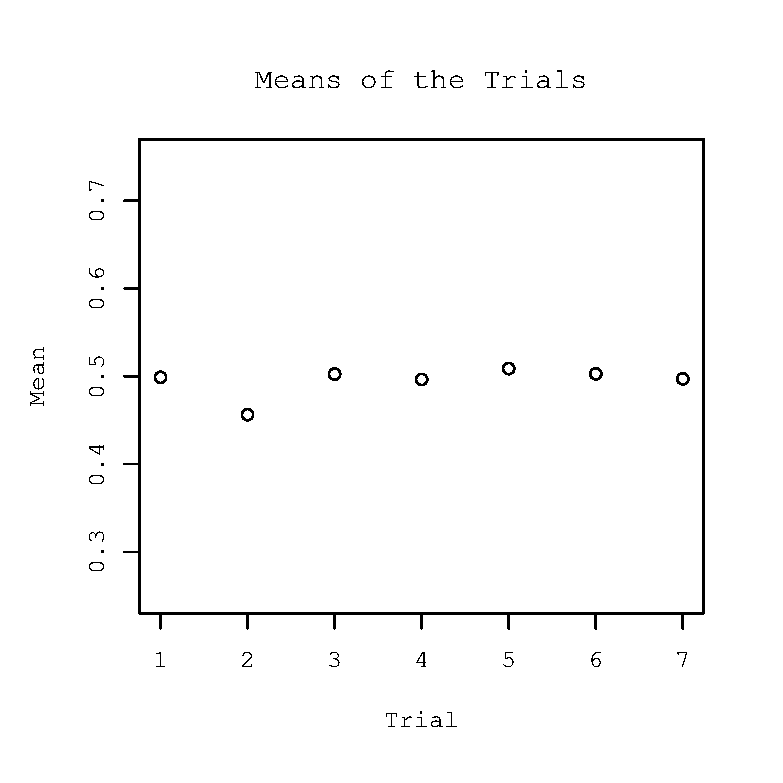
\includegraphics[height=3in]{centralLimitMeans}}
  \caption{The sample means of each of the seven  trials from Figures
    \ref{fig:centralLimitOne} to \ref{fig:centralLimitSeven}. The sample
    means from all of the trials is relatively constant.}
  \label{fig:centralLimitMeans}
\end{figure}

\begin{figure}[htp]
  \centerline{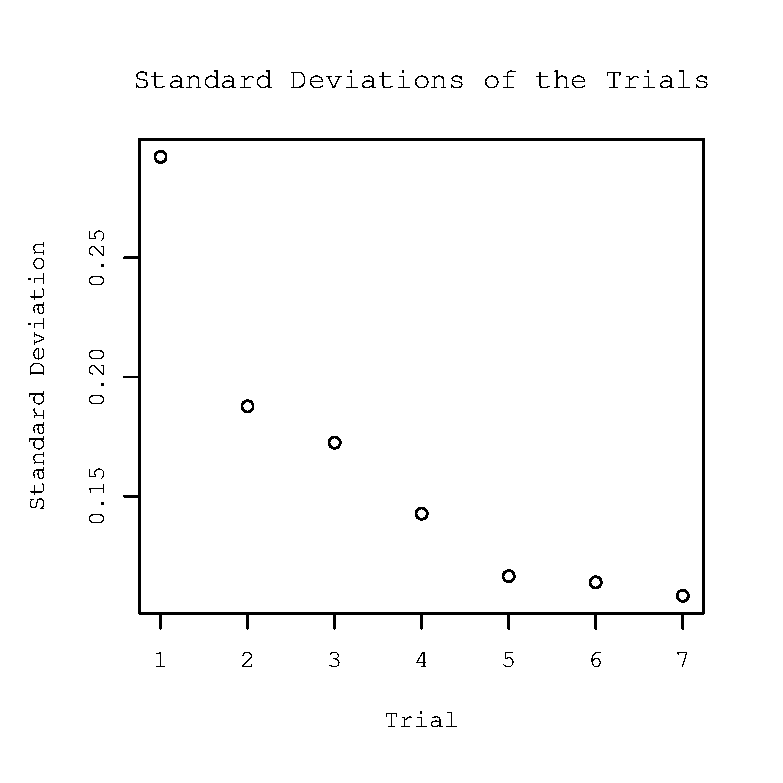
\includegraphics[height=3in]{centralLimitSTD}}
  \caption{The sample standard deviations of each of the seven trials
    from Figures \ref{fig:centralLimitOne} to \ref{fig:centralLimitSeven}.
    The sample standard deviations from all of the trials decreases
    like one over the square root of the sample size.}
  \label{fig:centralLimitSTD}
\end{figure}

In Figures \ref{fig:centralLimitMeans} and \ref{fig:centralLimitSTD}
the sample means and sample standard deviations from the results in
Figures \ref{fig:centralLimitOne} through \ref{fig:centralLimitSeven}
are shown. For each case the result of each trial was recorded and the
sample means and sample standard deviations from each case were
calculated. Overall, the means from each case are close to one
half. At the same time, the sample standard deviations from each set
of trials decreases like one over the square root of the sample size.


\begin{assignment}
  Given the following measurements, find the sample mean and find an
  estimate for the variance and the standard deviation of the sample
  mean.
  \begin{center}
    \begin{tabular}{rrrrrr}
      17 & 18 & 9 & 41 & 46 & 16 \\
      34 & 39 & 9 & 9  & 14 & 12 \\
      19 & 8      
    \end{tabular}
  \end{center}

\end{assignment}

\if y\solutions

\textbf{Solution:}

The sample mean can be calculated using equation
\ref{eqn:sampleObservations},
\begin{eqnarray*}
  \bar{x} & \approx & 20.79.
\end{eqnarray*}
The sample variance can be calculated using equation
\ref{eqn:sampleVariance}, 
\begin{eqnarray*}
  s^2_x & \approx & 177.10.
\end{eqnarray*}
The variance of the sample mean can be approximated using the sample
variance and Equation (\ref{eqn:varSampleMean}),
\begin{eqnarray*}
  \sigma^2_{\bar{x}} & \approx & \frac{s^2_x}{14},\\
    & \approx & 12.65.
\end{eqnarray*}
Finally, the standard deviation of the sample mean is found by taking
the square root of the variance,
\begin{eqnarray*}
  \sigma_{\bar{x}} & \approx & 3.56.
\end{eqnarray*}

\fi


\begin{assignment}
  Given the following measurements, find the sample mean and an
  estimate for the variance and the standard deviation of the sample
  mean.
  \begin{center}
    \begin{tabular}{rrrrrr}
       1.5 & 7.0 & 0.6 & 4.5 & 3.7 & 5.7 \\
       8.0 & 1.6 & 3.8 & 2.7 & 2.0 & 7.1
    \end{tabular}
  \end{center}
\end{assignment}

\if y\solutions

\textbf{Solution:}

The sample mean can be calculated using equation
\ref{eqn:sampleObservations},
\begin{eqnarray*}
  \bar{x} & \approx & 4.02.
\end{eqnarray*}
The sample variance can be calculated using equation
\ref{eqn:sampleVariance}, 
\begin{eqnarray*}
  s^2_x & \approx & 6.10.
\end{eqnarray*}
The variance of the sample mean can be approximated using the sample
variance and Equation (\ref{eqn:varSampleMean}),
\begin{eqnarray*}
  \sigma^2_{\bar{x}} & \approx & \frac{s^2_x}{12},\\
    & \approx & 0.51.
\end{eqnarray*}
Finally, the standard deviation of the sample mean is found by taking
the square root of the variance,
\begin{eqnarray*}
  \sigma_{\bar{x}} & \approx & 0.71.
\end{eqnarray*}

\fi



\section{Confidence Intervals} 
\label{section:confidenceIntervals}

Our goal is to determine the mean of a random variable based on a set
of observations.  Given a set of observations the sample mean can be
calculated and a sample standard deviation can be calculated. From
theorem \ref{thm:centralLimit} the sample mean can be approximated as
a normally distributed random variable, and an estimate for the
standard deviation for the mean can be calculated using the result in
Equation (\ref{eqn:sdSampleMean}).

The true mean of a random variable cannot be calculated.  The sample
mean is a collection of observations from a random variable, and the
sample mean can be used to approximate the true mean. Since the
observations have a random aspect to them it is possible that all of
the observations could be biased in one direction. It may be unlikely
that this could be the case, but it is possible. For this reason the
location of the true mean must be discussed in terms of the
probability that it is within a range of possible values.


\begin{figure}[tb]
  \centerline{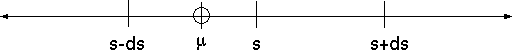
\includegraphics[width=4in]{confidence}}
  \caption{We determine an interval around the sample mean so that the
    probability that the true mean is within the interval is a
    predetermined, fixed number.}
  \label{fig:confidenceInterval}
\end{figure}


The true mean is not known, and a range of numbers in which the true
mean occurs cannot be definitely determined. Instead, a range of
numbers in which the true mean \textit{likely} occurs can be
determined, see Figure \ref{fig:confidenceInterval}.  There will be
some probability that the true mean falls outside of the interval, but
the probability that the true mean is outside of the interval can be
kept as low as possible. The size and location of the interval depends
on the probability density function describing the sample mean.

\begin{definition}
  The \textbf{confidence interval} is a range of numbers in which
  there is a fixed probability that the true mean of a random variable
  falls within the interval.
\end{definition}

\begin{definition}
  The \textbf{confidence level} is the probability that the true mean
  falls within the confidence interval. The probability is often
  denoted as $\alpha$.
\end{definition}

To determine the confidence interval the probability that the sample
mean is close to the true mean is examined. The problem is worked
backwards to determine an estimate for the location of the true mean
in terms of the sample mean. This approach may seem backwards at
first, but from the Central Limit Theorem an estimate of the
probability distribution of the sample mean can more easily express
the sample mean in terms of the true mean rather than vice versa.

Given a sequence of observations,
\begin{eqnarray*}
  x_1,~x_2,~x_3,\ldots,x_n,
\end{eqnarray*}
the sample mean, $\bar{x}$, and sample standard deviation, $s_{\rm
  x}$, can be determined using equations (\ref{eqn:sampleMean}) and
(\ref{eqn:sampleStandardDeviation}). The sample mean is a sum of
random variables so it is a random variable itself. From the Central
Limit Theorem it is approximated as a normally distributed random
variable with mean $\mu_{\rm x}$ and standard deviation $\sigma_{\rm
  x}/\sqrt{n}$.  The mean and standard deviation, $\mu_{\rm x}$ and
$\sigma_{\rm x}$, is not known. The value of $\sigma_{\rm x}$ is
approximated using the sample standard deviation, $s_{\rm x}$.


First, an interval is determined. The interval is centered on
$\mu_{\rm x}$.  The left side of the interval is located at $\mu_{\rm
  x}-\delta$, and the right side of the interval is located at
$\mu_{\rm x}+\delta$. (The value of $\delta$ is one half the length of
the entire interval.) The probability that the sample mean is located
within the interval should be equal to the confidence level,
\begin{eqnarray}
  \label{eqn:confIntervalStart}
  \alpha & = & \int^{\mu_{\rm x}+\delta}_{\mu_{\rm x}-\delta}
  \frac{1}{\sqrt{2\pi}\sigma_{\rm x}/\sqrt{n}} 
  e^{-(x-\mu_{\rm x})^2/(2\sigma_{\rm x}^2/n)}~dx.
\end{eqnarray}
Using a $u$-substitution,
\begin{eqnarray*}
  z & = & \frac{x-\mu_{\rm x}}{\sigma_{\rm x}/\sqrt{n}},
\end{eqnarray*}
Equation (\ref{eqn:confIntervalStart}) can be written as
\begin{eqnarray}
  \label{eqn:confidenceIntervalStandard}
  \alpha & = &
  \int^{\delta/(\sigma_{\rm x}/\sqrt{n})}_{-\delta/(\sigma_{\rm x}/\sqrt{n})} 
  \frac{1}{\sqrt{2\pi}} e^{-z^2/2}~dz.
\end{eqnarray}

Unfortunately, a closed form solution to the integral is not known,
and the value of the integral must be approximated. The goal is to
determine the value of $\delta$ given $\alpha$. In practice what is
done is make the substitution
\begin{eqnarray}
  \label{eqn:defineZStar}
  z^* & = & \frac{\delta}{\sigma_{\rm x}/\sqrt{n}},
\end{eqnarray}
and Equation (\ref{eqn:confidenceIntervalStandard}) can be expressed
as
\begin{eqnarray*}
  \alpha & = &
  \int^{z^*}_{-z^*} \frac{1}{\sqrt{2\pi}} e^{-z^2/2}~dz.  
\end{eqnarray*}
Good approximations for the value of $z^*$ exist and are listed in
Table \ref{tab:confidenceZVals}. Once $z^*$ is determined the value of
$\delta$ can be found by solving for $\delta$ in equation
(\ref{eqn:defineZStar}),
\begin{eqnarray}
  \label{eqn:widthCI}
  \delta & = & z^* \frac{\sigma_{\rm x}}{\sqrt{n}}.
\end{eqnarray}

\begin{table}[ht]
  \begin{center}
    \begin{tabular}{cc}
      Confidence Level ($\alpha$) & $z^*$ \\ \hline 
      .90 & 1.644854 \\
      .95 & 1.959964 \\
      .99 & 2.575829
    \end{tabular}    
  \end{center}
  \caption{Approximations for $z^*$ for different confidence levels, $\alpha$.}
  \label{tab:confidenceZVals}
\end{table}

It is important to note that there is a problem with using equation
(\ref{eqn:widthCI}). Given a set of observations an approximation is
found for the standard deviation by using the sample standard
deviation. The sample standard deviation is determined by the
observations and hence is a random variable itself. The probability
distribution for the sample variation is known and is a $\chi^2$
distribution.  The distribution for the resulting mean is also known
and is a $t$-distribution.  These are topics that go beyond this brief
introduction, but it is important to realize that in practice the
confidence level should be approximated using a $t$-distribution. For
our purposes in this setting, though, the approximation from equation
(\ref{eqn:widthCI}) is a reasonable approximation.

An interval has been found around the true mean, and the sample mean
should lie in the interval with a known probability. The problem is
that the sample mean is known but the true mean is not known.
Fortunately, the relationships for the interval around the true mean
can be written in terms of the sample mean.

Equation (\ref{eqn:widthCI}) implies that the sample mean has a
probability of $\alpha$ to satisfy the relationship
\begin{eqnarray*}
  \begin{array}{rclcl}
    \mu_{\rm x} - \delta & < & \bar{x} & < & \mu_{\rm x} + \delta.
  \end{array}
\end{eqnarray*}
The left part of the relationship implies that
\begin{eqnarray}
  \label{eqn:upperBoundMu}
  \mu_{\rm x} & < & \bar{x} + \delta.
\end{eqnarray}
The right part of the relationship implies that
\begin{eqnarray}
  \label{eqn:lowerBoundMu}
   \bar{x} - \delta & < &  \mu_{\rm x}.
\end{eqnarray}
Taken together, equations (\ref{eqn:upperBoundMu}) and
(\ref{eqn:lowerBoundMu}), imply that there is a probability of
$\alpha$ that the true mean satisfies the relationship
\begin{eqnarray}
  \begin{array}{rclcl}
    \bar{x} - \delta & < & \mu_{\rm x} & < & \bar{x} + \delta.
   \end{array}
\end{eqnarray}


Cavendish's observations are used as an example for the relative
density of the earth given in Table \ref{table:cavendish}. The sample
mean of the data is
\begin{eqnarray*}
  \bar{x} & \approx & 5.45,
\end{eqnarray*}
and the sample standard deviation is 
\begin{eqnarray*}
  s_{\rm x} & \approx & .22.
\end{eqnarray*}
There are 29 observations and to find the 95\% confidence level so
\begin{eqnarray*}
  \delta & \approx & 1.65 \frac{.22}{\sqrt{29}}, \\
         & \approx & .067.
\end{eqnarray*}
The 95\% confidence interval is between 5.38 and 5.52. There is a
probability of .95 that the true mean is between 5.38 and 5.52.


\begin{assignment}
  Find the 95\% confidence interval for the mean of a random variable
  with the following samples:
  \begin{center}
    \begin{tabular}{rrrrrr}
      17 & 18 & 9 & 41 & 46 & 16 \\
      34 & 39 & 9 & 9  & 14 & 12 \\
      19 & 8      
    \end{tabular}
  \end{center}
\end{assignment}

\if y\solutions

\textbf{Solution:}

The sample mean is
\begin{eqnarray*}
  \bar{x} & \approx & 20.79.
\end{eqnarray*}
The variance of the sample  is 
\begin{eqnarray*}
  s^2_{\mathrm x} & \approx & 177.10.
\end{eqnarray*}
From Table \ref{tab:confidenceZVals} the value of $z^*$ is
\begin{eqnarray*}
  z^* & \approx & 1.959964.
\end{eqnarray*}
From Equation (\ref{eqn:widthCI}) the width of the confidence interval
can be found,
\begin{eqnarray*}
  \delta & = & z^* \frac{\sigma_{\rm x}}{\sqrt{n}}, \\
  & \approx & 1.959964 \frac{\sqrt{177.10}}{\sqrt{14}}, \\
  & \approx & 6.97.
\end{eqnarray*}
There is a probability of 0.95 that the true mean is in the interval
\begin{eqnarray*}
  \begin{array}{r@{~\leq~}c@{~\leq~}l}
  20.79-6.97 & \mu_x & 20.79+6.97, \\
  13.81 & \mu_x & 27.76.
  \end{array}
\end{eqnarray*}

\fi

\begin{assignment}
  Find the 95\% confidence interval for the mean of a random variable
  with the following samples:
  \begin{center}
    \begin{tabular}{rrrrrr}
       1.5 & 7.0 & 0.6 & 4.5 & 3.7 & 5.7 \\
       8.0 & 1.6 & 3.8 & 2.7 & 2.0 & 7.1
    \end{tabular}
  \end{center}
\end{assignment}

\if y\solutions

\textbf{Solution:}

The sample mean is
\begin{eqnarray*}
  \bar{x} & \approx & 4.02.
\end{eqnarray*}
The variance of the sample  is 
\begin{eqnarray*}
  s^2_{\mathrm x} & \approx & 6.10.
\end{eqnarray*}
From Table \ref{tab:confidenceZVals} the value of $z^*$ is
\begin{eqnarray*}
  z^* & \approx & 1.959964.
\end{eqnarray*}
From Equation (\ref{eqn:widthCI}) the width of the confidence interval
can be found,
\begin{eqnarray*}
  \delta & = & z^* \frac{\sigma_{\rm x}}{\sqrt{n}}, \\
  & \approx & 1.959964 \frac{\sqrt{6.10}}{\sqrt{12}}, \\
  & \approx & 1.40.
\end{eqnarray*}
There is a probability of 0.95 that the true mean is in the interval
\begin{eqnarray*}
  \begin{array}{r@{~\leq~}c@{~\leq~}l}
  4.02-1.40 & \mu_x & 4.02+1.40, \\
  2.62 & \mu_x & 5.41.
  \end{array}
\end{eqnarray*}

\fi



\begin{assignment}
  You are asked to do an experiment and want to know the mean of a set
  of observations. In previous, similar studies the sample standard
  deviation has been reported to be in the range of between 0.12 and
  0.18. Find an estimate of the number of observations that are
  necessary so that the 95\% confidence level will be $\pm 0.01$ of
  the sample mean that you will calculate. How many observations are
  needed for the 95\% confidence level to be $\pm 0.005$ of the sample
  mean?
\end{assignment}

\if y\solutions

\textbf{Solution:}

From Equation (\ref{eqn:widthCI}) the width of the confidence interval
can be found,
\begin{eqnarray*}
  \delta & = & z^* \frac{\sigma_{\rm x}}{\sqrt{n}}.
\end{eqnarray*}
We are given the following:
\begin{eqnarray*}
  \delta & = & 0.01, \\
  z^* & \approx & 1.959964,
\end{eqnarray*}
and the standard deviation is between 0.12 and 0.18. Solving the expression
for $n$ we get
\begin{eqnarray*}
  \sqrt{n} & = & z^* \frac{\sigma_{\rm x}}{\delta}, \\
  n & = & \lp z^* \rp^2 \frac{\sigma^2_{\rm x}}{\delta^2}.
\end{eqnarray*}
The largest this can be is when the standard deviation is 0.18. An
approximation for the number is
\begin{eqnarray*}
  n & \approx &  1.959964^2 \frac{0.18^2}{.01^2}, \\
  n & \approx & 1244.6.
\end{eqnarray*}
The number of trials that should be used is 1245.

If the width of the interval is 0.005 then the previous expression
reduces to 4978.5. For an error of $\pm 0.005$, 4979 trials should be
used. (It went up by a factor of four.)


\fi



\section{Linear Regression}

The idea behind linear regression is that a set of observations
consisting of two or more measurements for each observation is found,
and the relationship between the measurements is approximately linear.
Only two measurements per observation are examined here. In each
observation the two measurements are denoted $(x_i,y_i)$. It is
assumed that $x_i$ is the independent variable and $y_i$ is the
independent variable. It is also assumed that the value of $x_i$ is
known to a much higher degree of precision than $y_i$.

\begin{figure}[tb]
  \centerline{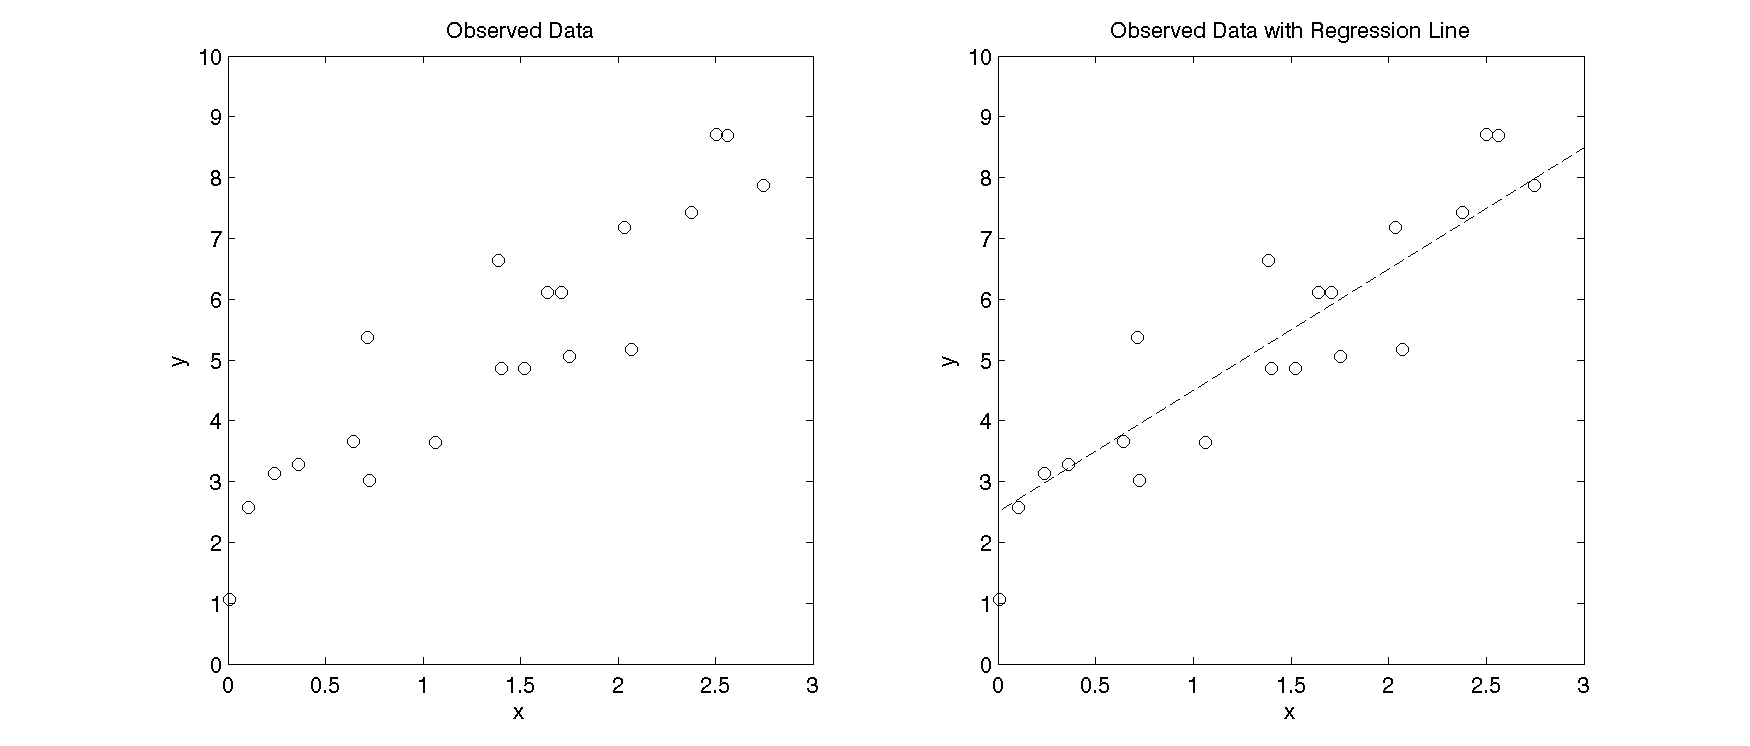
\includegraphics[width=5.5in]{linearSample}}
  \caption{The left hand side represents a number of
    measurements. Each circle comes from a single measurement. The
    right hand side is the same measurements with an approximation of
    the best straight line that represents the relationship between
    the data pairs.}
  \label{fig:linearRegressionSample}
\end{figure}

The relationship between $x_i$ and $y_i$ is assumed to be
approximately linear,
\begin{eqnarray*}
  y_i & \approx & m x_i + b.
\end{eqnarray*}
The goal is to find approximations to $m$ and $b$ given a set of
measurements.  An example can be seen in Figure
\ref{fig:linearRegressionSample}. In the left hand side of the figure
a graphical set of measurements where each circle represents a data
pair, $(x_i,y_i)$. In the right hand side of the figure the dotted
line is an approximation of the straight line that best represents the
relationship between the $x$ values and the $y$ values.





Few actual relationships are linear, but fortunately, many
relationships can be transformed to appear linear.  Two examples of
how to transform certain kinds of relationships to appear linear are
given. The details about how to find a ``best'' straight line to
approximate the data is then examined.  Finally, some of the issues
associated with the process are examined.



\subsection{Exponential Relationships}

The relationships between physical quantities take on a variety of
different forms. Some general types of relationships are common enough
that standard approaches have been developed. One example is a
relationship between two quantities, $S$ and $t$, that is an
exponential relationship,
\begin{eqnarray*}
  S & = & A \; c^{t},
\end{eqnarray*}
where $A$ and $c$ are constants.  The relationship between $S$ and $t$
can be transformed into a linear relationship by first taking the
logarithm of both sides:
\begin{eqnarray*}
  \ln(S) & = & \ln\lp A \; c^{t} \rp.
\end{eqnarray*}
From the properties of the logarithm the relationship can be rewritten
in a different form,
\begin{eqnarray*}
  \ln(S) & = & \ln\lp A\rp + \ln\lp c^{t} \rp, \\
         & = & \ln\lp A\rp + \ln\lp c\rp \cdot t.
\end{eqnarray*}
The relationship between $S$ and $t$ is not linear, but the
relationship between $\ln(S)$ and $t$ is linear,
\begin{eqnarray*}
  \underbrace{\ln(S)}_y
  & = & 
  \underbrace{\ln\lp A\rp}_b + 
  \underbrace{\ln\lp c\rp}_m \cdot \underbrace{t}_x, 
\end{eqnarray*}
the result is a linear relationship in the form
\begin{eqnarray*}
  y & = & b + mx.
\end{eqnarray*}

An example of the  relationship
\begin{eqnarray*}
  S & = & 3.5\; \lp .8 \rp^{t}
\end{eqnarray*}
is examined.  A graph of the relationship is seen in the left hand
side of Figure \ref{fig:semilog} with samples at discrete values of
$t$. If you take the same numbers and plot the logarithm of $S$ versus
$t$ the relationship is a straight line. Note that the slope of the
linear relationship is negative. This is because the logarithm of
$0.8$ is negative. A negative slope indicates exponential decay, and a
positive slope indicates exponential growth.

\begin{figure}[tb]
  \centerline{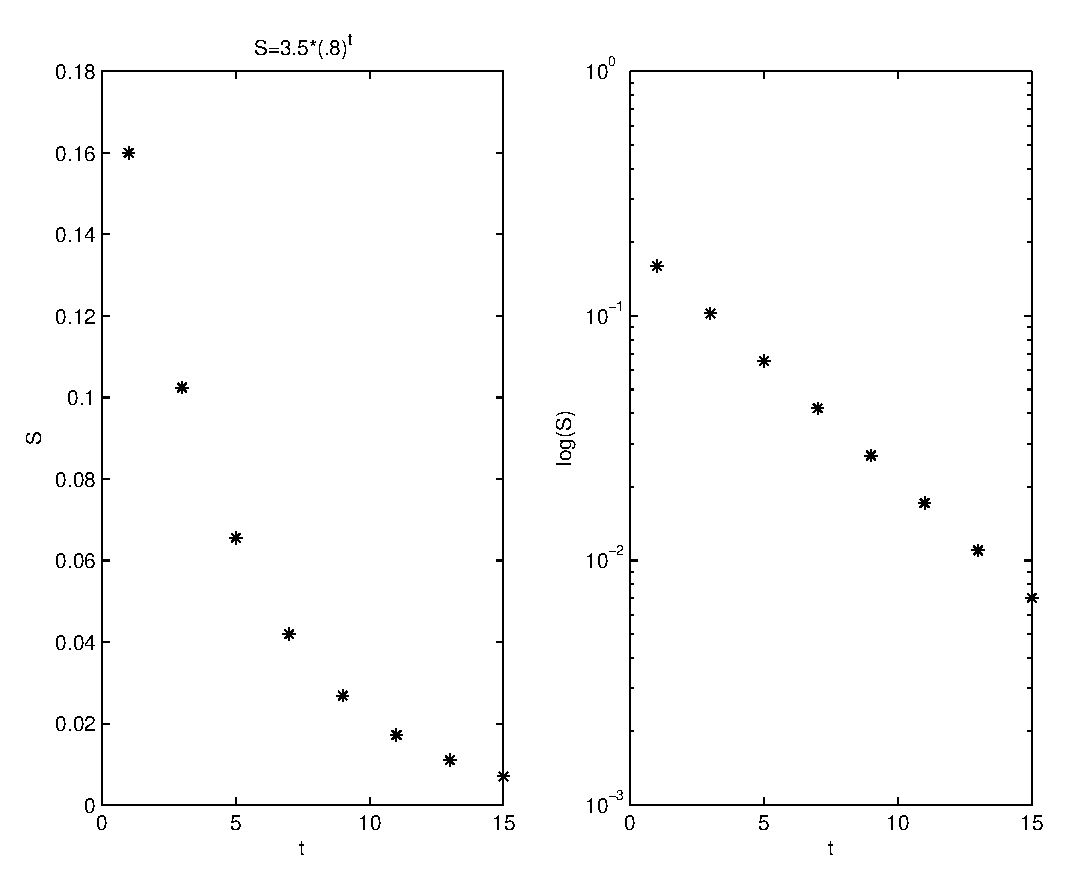
\includegraphics[height=2.5in]{semilog}}
  \caption{An exponential relationship can be transformed into a
    linear relation by looking at the logarithm of the dependent
    variable.}
  \label{fig:semilog}
\end{figure}




\subsection{Power Relationships}

Another common relationship between two variables is a power
relationship. This is also sometimes refered to as allometry. A power
relationship is of the form
\begin{eqnarray*}
  S & = & A t^{r},
\end{eqnarray*}
where $A$ and $r$ are constants.  

This kind of relationship can be turned into a linear relationship by
first taking the logarithm of both sides:
\begin{eqnarray*}
  \ln(S) & = & \ln\lp A t^r \rp.
\end{eqnarray*}
Again, the properties of the logarithm allow the different parts of
the expression on the right hand side to be separated,
\begin{eqnarray*}
\ln(S)  & = & \ln\lp A \rp + \ln\lp t^r \rp, \\
        & = & \ln\lp A\rp + r \ln\lp t \rp. 
\end{eqnarray*}
The relationship between $S$ and $t$ is not a linear relationship, but
the relationship between $\ln(S)$ and $\ln(t)$ is linear. The value of
$A$ and $r$ is a constant so a clever substitution will result in a
linear relationship,
\begin{eqnarray*}
  \underbrace{\ln(S)}_y
  & = & 
  \underbrace{\ln\lp A\rp}_b + 
  \underbrace{r}_m \underbrace{\ln\lp t \rp}_x. \\
\end{eqnarray*}
The relationship is now in the form
\begin{eqnarray*}
  y & = & b + mx.
\end{eqnarray*}

An example of the relationship
\begin{eqnarray*}
  S & = & 0.2 \cdot t^{4.5}
\end{eqnarray*}
is examined.  A graph of the relationship is seen in the left hand
side of Figure \ref{fig:loglog} with samples at discrete values of
$t$.  If you take the same numbers and plot the logarithm of $S$
versus the logarithm of $t$ the relationship is a straight line.
Notice that the slope of the linear relationship is positive.  The
value of $r$ is positive so the slope of the line for the logarithms
is positive.

\begin{figure}[tb]
  \centerline{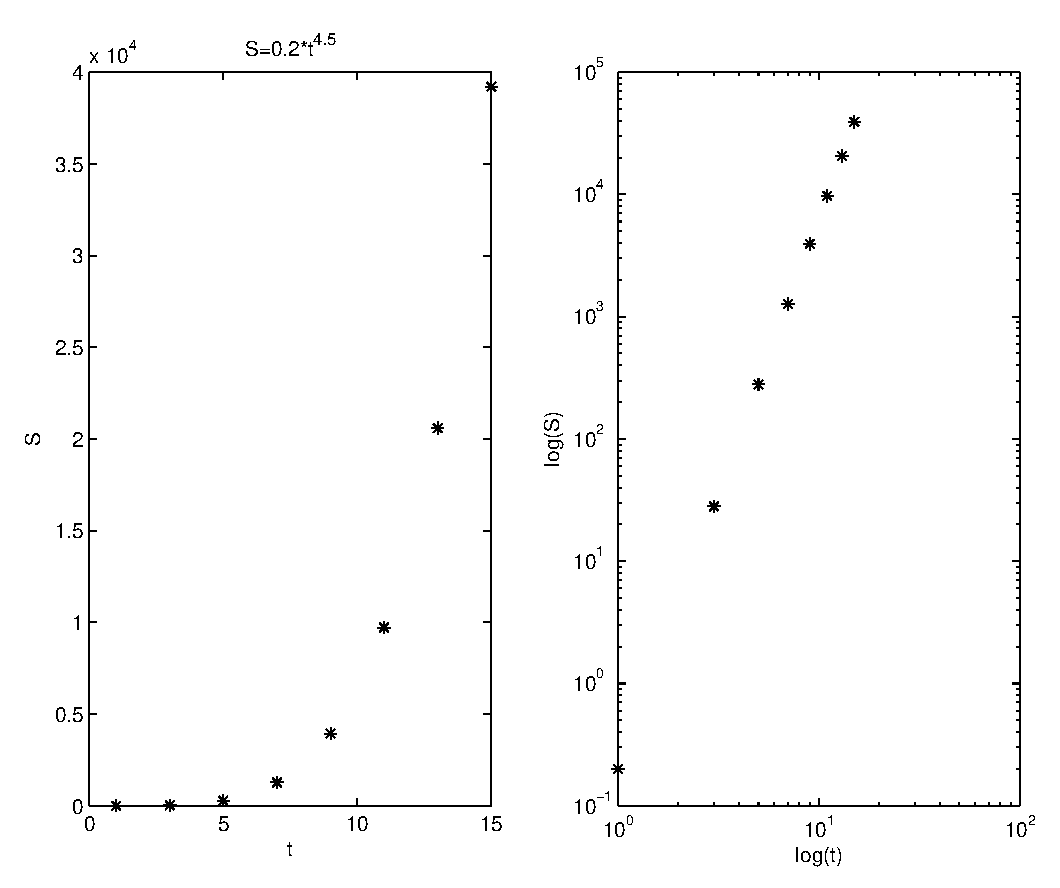
\includegraphics[height=2.5in]{loglog}}
  \caption{A power relationship can be transformed into a linear
    relation by looking at the logarithm of both the independent and
    the dependent variable.}
  \label{fig:loglog}
\end{figure}




\subsection{Correlation}

Given a set of observations the next question is how to decide if the
variation in one variable can be described as a linear relationship on
another variable. One way to do this is the ``correlation'' between
two variables.  The correlation of a data set is a number between
minus one and one. The farther the number is from zero the better the
stronger the case for a linear relationship. For example, if the
correlation is one or minus one then it is likely a linear
relationship.

It is assumed that a set of data points from a set of observations has
been recorded. The data points can be expressed as the following:
\begin{eqnarray}
  \label{eqn:dataPairs}
  x_1 & y_1, \\
  x_2 & y_2, \nonumber \\
  x_3 & y_3, \nonumber \\
  \vdots & \vdots \nonumber \\
  x_n & y_n. \nonumber 
\end{eqnarray}
The values of $x$ are arbitrarily called the ``independent variable''
and the values of $y$ are the ``dependent variable.''  Great care is
required in that this is a mathematical description. A mathematical
relationship between two variables does not imply any link of
causation between them.

Before defining the correlation some intermediate definitions are
required.  First, the independent and dependent variables are examined
separately.  Looking at the independent variables,
\begin{eqnarray*}
  x_1,~x_2,~x_3,\ldots,x_n,
\end{eqnarray*}
then this is a univariate data set on which the standard statistical
measurements can be defined.  The same thing is true of the dependent
variables,
\begin{eqnarray*}
  y_1,~y_2,~y_3,\ldots,y_n.
\end{eqnarray*}
Because there are two data sets notation to distinguish between the
two relevant statistics is needed.

\begin{definition}
  The sample mean of the dependent variable is 
  \begin{eqnarray}
    \bar{x} & = & \frac{1}{n} \lp x_1 + x_2 + x_3 + \cdots + x_n \rp, \\
    & = & \frac{1}{n} \sum^n_{k=1} x_k. \nonumber
  \end{eqnarray}
  This is the exact same expression as given in equation
  (\ref{eqn:sampleMean}).
\end{definition}

\begin{definition}
  The sample mean of the independent variable is 
  \begin{eqnarray}
    \bar{y} & = & \frac{1}{n} \lp y_1 + y_2 + y_3 + \cdots + y_n \rp, \\
    & = & \frac{1}{n} \sum^n_{k=1} y_k. \nonumber
  \end{eqnarray}
\end{definition}

\begin{definition}
  The sample variance of the independent variable is
  \begin{eqnarray}
    s^2_{\rm x} & = & \frac{1}{n-1} \sum^n_{k=1} \lp x_k - \bar{x} \rp^2.
  \end{eqnarray}  
  This is the exact same expression as given in equation
  (\ref{eqn:sampleVariance}).
  The sample standard deviation of the independent variable is
  \begin{eqnarray*}
    s_{\rm x} & = & \sqrt{s^2_{\rm x}}.
  \end{eqnarray*}
\end{definition}

\begin{definition}
  The sample variance of the dependent variable is
  \begin{eqnarray}
    s^2_{\rm y} & = & \frac{1}{n-1} \sum^n_{k=1} \lp y_k - \bar{y} \rp^2.
  \end{eqnarray}  
  The sample standard deviation of the dependent variable is
  \begin{eqnarray*}
    s_{\rm y} & = & \sqrt{s^2_{\rm y}}.
  \end{eqnarray*}
\end{definition}

The next step is to draw a connection between the independent and
dependent variables. The covariance and the correlation is defined in
terms of the covariance and the standard deviations.

\begin{definition}
  The sample covariance of the independent and dependent variables is
  \begin{eqnarray}
    \label{eqn:covariance}
    \mathrm{Cov}(x,y) & = & \frac{1}{n-1} \sum^n_{k=1} (x_k-\bar{x})(y_k-\bar{y}).
  \end{eqnarray}
\end{definition}

\begin{definition}
  The sample correlation between the independent and dependent variables is
  \begin{eqnarray*}
    r & = & \frac{\mathrm{Cov}(x,y)}{s_{\rm x} \cdot s_{\rm y}}.
  \end{eqnarray*}
\end{definition}

The sample correlation is always a number between minus one and one.
It is not obvious from the definition but is explored in some of the
exercises given below. The focus is on the interpretation of the
correlation. Different data sets are plotted in Figure
\ref{fig:correlation} that have different correlations. For each plot
the data point, $(x_k,y_k)$, is plotted in the plane with the
dependent variable on the horizontal axis and the independent variable
on the vertical axis. This kind of plot is called a ``scatter plot.''


\begin{figure}[tb]
  \centerline{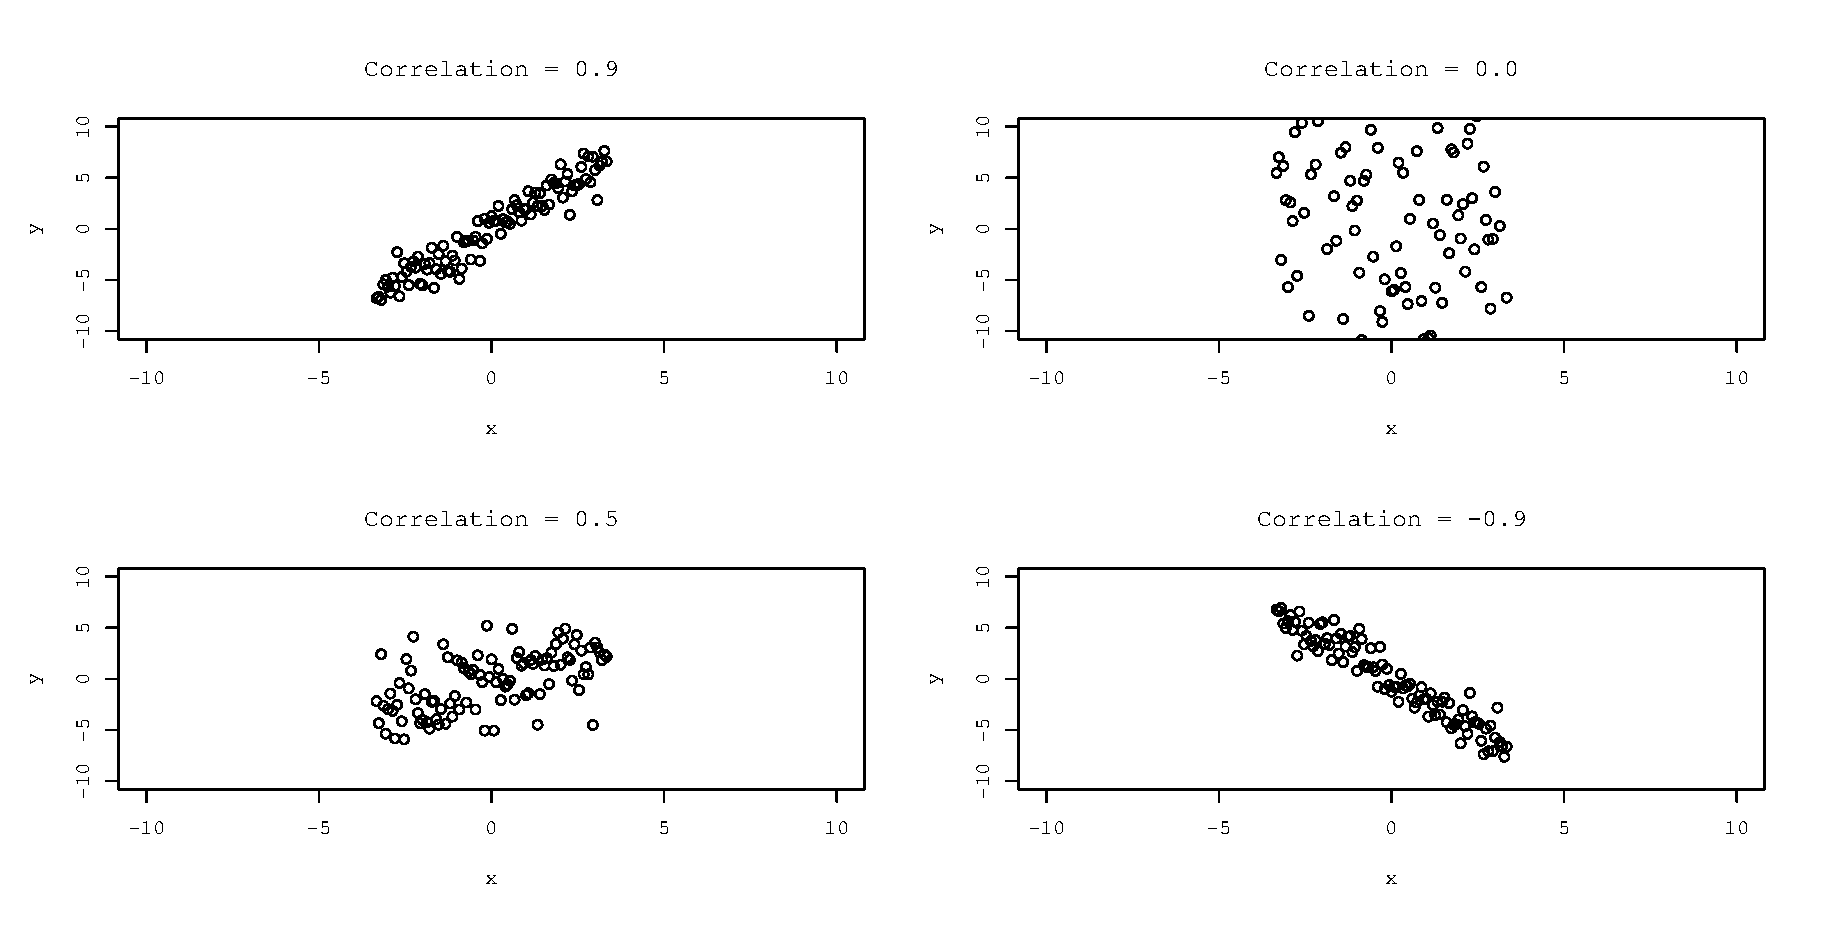
\includegraphics[height=2.5in]{correlation}}
  \caption{The correlation of a set of numbers is a number between
    minus one and one. The closer the relationship is to one or minus
    one the more the variance between the two can be attributed to a
    linear relationship.}
  \label{fig:correlation}
\end{figure}

The plot in the upper left corner of Figure \ref{fig:correlation}
shows a data set whose sample correlation is close to 0.9. There is a
strong linear relationship, and the two variables have a positive
association. As the dependent variable increases the independent
variable also increases. In the bottom left corner of Figure
\ref{fig:correlation} the sample correlation is close to 0.5.  The
data has a positive association, but there is not as strong a linear
relationship. In the top right corner of Figure \ref{fig:correlation}
the sample correlation is close to zero. There is no obvious
relationship between the two variables. Finally, in the bottom right
corner of Figure \ref{fig:correlation} the sample correlation is close
to -0.9. There is a strong linear relationship, but it is a negative
association. As the independent variable increases the dependent
variable decreases.



It is important to note that the correlation alone is not necessarily
meaningful.  An example is given in Figures \ref{fig:correlation1}
through \ref{fig:correlation4}. In the first figure, Figure
\ref{fig:correlation1}, the data points are plotted as a scatter plot.
In the second figure a ``good'' straight line is added that is a good
approximation of the data. The sample correlation of the data sample
is approximately 0.96 which indicates a strong linear relationship.

\begin{figure}[tb]
  \centerline{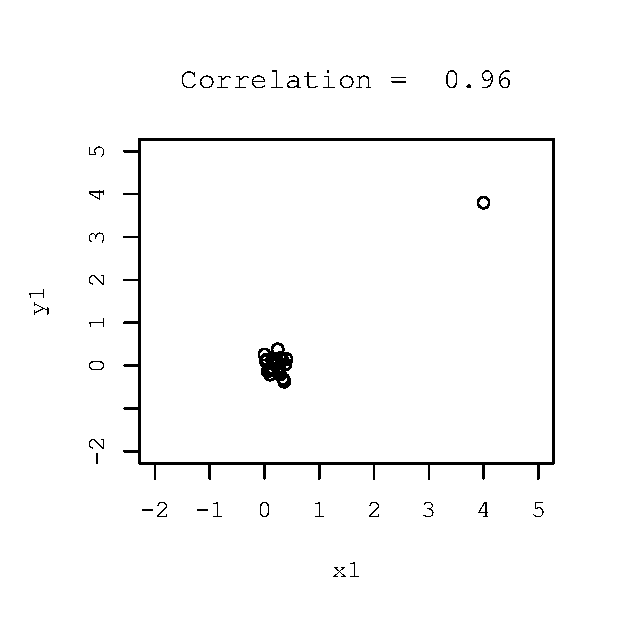
\includegraphics[height=3in]{correlation1}}
  \caption{The correlation of a set of numbers.}
  \label{fig:correlation1}
\end{figure}

\begin{figure}[tb]
  \centerline{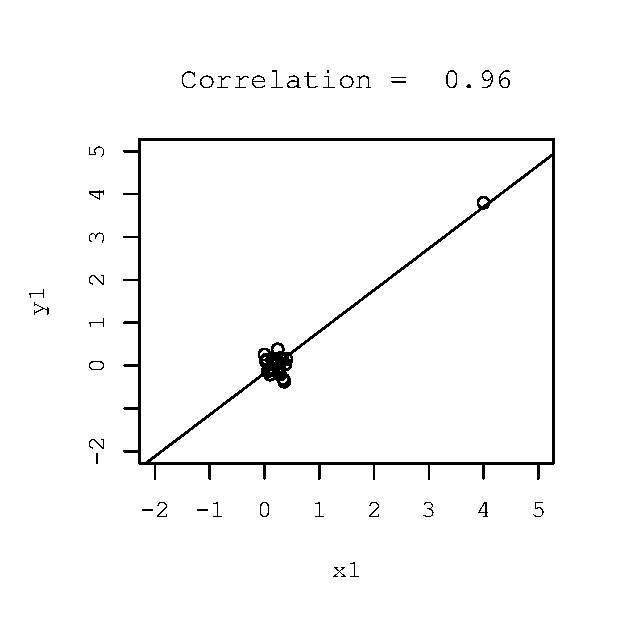
\includegraphics[height=3in]{correlation2}}
  \caption{The correlation of the set of numbers from the previous
    figure with a ``good'' straight line approximation of the data.}
  \label{fig:correlation2}
\end{figure}

One of the data points in this example is different from the others,
and it does not follow the same overall pattern as the other data
points. The data point near $(4,4)$ does not follow the same trend as
the other data points. In Figures \ref{fig:correlation3} through
\ref{fig:correlation4} this point is removed and the sample
correlation is examined. A new ``good'' straight line is plotted.
Without the extra point the correlation is close to zero, and the
straight line approximation is dramatically different.

\begin{figure}[tb]
  \centerline{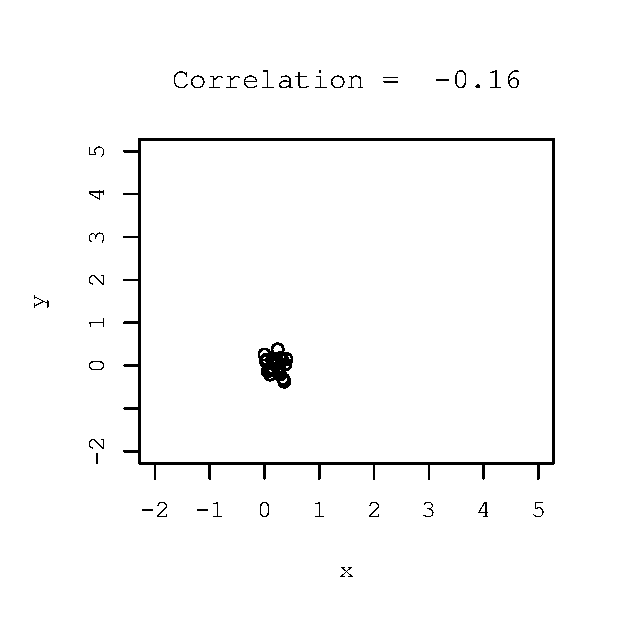
\includegraphics[height=3in]{correlation3}}
  \caption{The correlation of the set of numbers from the previous
    figure with the one outlier removed.}
  \label{fig:correlation3}
\end{figure}

\begin{figure}[tb]
  \centerline{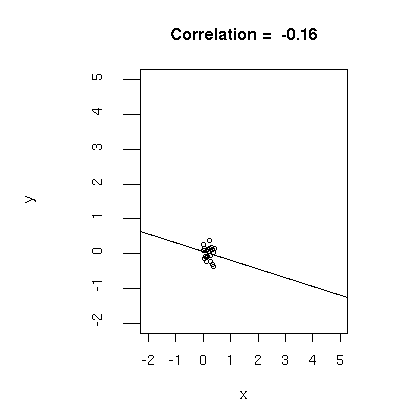
\includegraphics[height=3in]{correlation4}}
  \caption{The correlation of the set of numbers from the previous
    figure with a ``good'' straight line approximation of the data.}
  \label{fig:correlation4}
\end{figure}

The important lesson here is that simply finding a correlation is not
an adequate way by itself to justify a conclusion that a relationship
is linear. It is important to note that in the previous example one
point in the data set made a big difference to the overall analysis.
This is a common enough problem that it is something that is discussed
when examining a given data set. Two new definitions are necessary.

\begin{definition}
  An observation that does not follow the overall pattern is called an
  \textbf{outlier}.
\end{definition}

\begin{definition}
  A point that changes the overall statistics to a large degree if it
  is removed is an \textbf{influential} point.
\end{definition}

\begin{assignment}
  Find the correlation of the following data points:
  \begin{eqnarray*}
    0.00, 1.00 \\
    1.00, 1.09 \\
    2.00, 1.17 \\
    3.00, 1.23 \\
    4.00, 1.28 \\
    5.00, 1.31
  \end{eqnarray*}
\textit{Answer: approximately 0.98.}
\end{assignment}

\if y\solutions

\textbf{Solution:}

The standard deviations are approximated by
\begin{eqnarray*}
  s_{\mathrm x} & \approx & 1.87, \\
  s_{\mathrm y} & \approx & 0.12.
\end{eqnarray*}
The covariance of the pairs is
\begin{eqnarray*}
  \mathrm{Cov}(x,y) & \approx & 0.218.
\end{eqnarray*}
The correlation is
\begin{eqnarray*}
  r & \approx & 0.98.
\end{eqnarray*}

\fi


\begin{assignment}
  Suppose that a set of observations are made,
  \begin{eqnarray*}
    x_1,~x_2,~x_3,\ldots,x_n.
  \end{eqnarray*}
  A new variable is defined by
  \begin{eqnarray*}
    y_k & = & m x_k + b,
  \end{eqnarray*}
  where $m$ and $b$ are constants. Show that the sample mean of the
  $y_k$'s is given by
  \begin{eqnarray*}
    \bar{y} & = & m \bar{x} + b.
  \end{eqnarray*}
\end{assignment}

\if y\solutions
\textbf{Solution:} 

From Equation (\ref{eqn:sampleMean}) the sample mean of the
new variable, $\bar{y}$, is
\begin{eqnarray*}
  \bar{y} & = & \frac{1}{n} (y_1 + y_2 + y_3 + \cdots + y_n), \\
  & = & \frac{1}{n} \lp (m x_1 + b) + (m x_2 + b) + (m x_3 + b) +
  \cdots + (m x_n + b) \rp, \\
  & = & \frac{1}{n} \lp m x_1 + m x_2 + m x_3 + \cdots + m x_n 
  + b + b + b + \cdots + b \rp, \\
  & = & \frac{1}{n} \lp m \lp \sum^n_{k=1} x_k \rp + n\cdot b \rp, \\
  & = & m \lp \frac{1}{n} \sum^n_{k=1} x_k \rp + b, \\
  & = & m \bar{x} + b.
\end{eqnarray*}

\fi

\begin{assignment}
  A set of observations results in data pairs given by
  \begin{eqnarray*}
    x_1 & y_1, \\
    x_2 & y_2, \\
    x_3 & y_3, \\
    \vdots & \vdots \\
    x_n & y_n.
  \end{eqnarray*}
  Two vectors can be defined by
  \begin{eqnarray*}
    \vec{x} & = & 
    \left[
      \begin{array}{c}
        x_1 - \bar{x} \\
        x_2 - \bar{x} \\
        x_3 - \bar{x} \\
        \vdots \\
        x_n - \bar{x}
      \end{array}
      \right],
  \end{eqnarray*}
  and
  \begin{eqnarray*}
    \vec{y} & = & 
    \left[
      \begin{array}{c}
        y_1 - \bar{y} \\
        y_2 - \bar{y} \\
        y_3 - \bar{y} \\
        \vdots \\
        y_n - \bar{y}
      \end{array}
      \right].
  \end{eqnarray*}
  Show that the sample covariance of the data set can be written as
  the dot product of the two vectors defined above divided by $n-1$.
  Find an expression for the cosine of the angle between the vectors,
  $\vec{x}$ and $\vec{y}$, in terms of the sample covariance and the
  sample standard deviations of the two variables. Finally, explain
  why the correlation is always a number between minus one and one.
\end{assignment}

\if y\solutions
\textbf{Solution:} 

The dot product of the two vectors is
\begin{eqnarray*}
  \vec{x}\cdot\vec{y} & = & (x_1-\bar{x})(y_1-\bar{y}) +
  (x_2-\bar{x})(y_2-\bar{y}) + \cdots + (x_n-\bar{x})(y_n-\bar{y}).
\end{eqnarray*}
After dividing this expression by $n-1$,
\begin{eqnarray*}
  \frac{1}{n-1} \vec{x}\cdot\vec{y} & = & 
  \frac{1}{n-1} \lp (x_1-\bar{x})(y_1-\bar{y}) +
  (x_2-\bar{x})(y_2-\bar{y}) + \cdots + (x_n-\bar{x})(y_n-\bar{y}) \rp, 
\end{eqnarray*}
the result is the same expression as given in Equation
(\ref{eqn:covariance}).

Note that the standard deviation of the independent variable is
\begin{eqnarray*}
  s_{\mathrm x} & = & \sqrt{ \frac{1}{n-1} 
  \lp (x_1-\bar{x})^2 + (x_2-\bar{x})^2 + \cdots + (x_n-\bar{x})^2 \rp} , \\
  & = & \sqrt{\frac{1}{n-1}} ~ \| \vec{x} \|.
\end{eqnarray*}
Likewise, a similar result holds for the dependent variable,
\begin{eqnarray*}
  s_{\mathrm y} & = & \sqrt{ \frac{1}{n-1} 
  \lp (y_1-\bar{y})^2 + (y_2-\bar{y})^2 + \cdots + (y_n-\bar{y})^2 \rp} , \\
  & = & \sqrt{\frac{1}{n-1}} ~ \| \vec{y} \|.
\end{eqnarray*}

From the definition of the dot product,
\begin{eqnarray*}
  \vec{x}\cdot\vec{y} & = & \|\vec{x}\| \, \|\vec{y}\| \, \cos(\theta),
\end{eqnarray*}
where $\theta$ is the angle between $\vec{x}$ and $\vec{y}$. Solving
the equation for the cosine gives
\begin{eqnarray*}
  \cos(\theta) & = & \frac{\vec{x}\cdot\vec{y}}{\|\vec{x}\| \, \|\vec{y}\|}.
\end{eqnarray*}
Multiplying the top and bottom of the right hand of this expression by
$\frac{1}{n-1}$ gives
\begin{eqnarray*}
    \cos(\theta) & = & \frac{\frac{1}{n-1}\vec{x}\cdot\vec{y}}{
      \frac{1}{n-1} \|\vec{x}\| \, \|\vec{y}\|}, \\
    & = & \frac{\frac{1}{n-1}\vec{x}\cdot\vec{y}}{
      \sqrt{\frac{1}{n-1}} \|\vec{x}\| \, \sqrt{\frac{1}{n-1}} \|\vec{y}\|}, \\
    & = & \frac{\mathrm{Cov}(x,y)}{s_{\rm x} \cdot s_{\rm y}}.
\end{eqnarray*}

The correlation between two sets of samples is the same as finding the
cosine of the angle between $\vec{x}$ and $\vec{y}$. The cosine of an
angle is always between -1 and 1, so the correlation is always between
-1 and 1.

\fi

\begin{assignment}
  Use the two previous assignments to show that if $y_k=m x_k+b$ where
  $m$ and $b$ are constants then the sample correlation is one if $m$
  is positive and is minus one if $m$ is negative. What happens when
  $m$ is zero?
\end{assignment}

\if y\solutions

\textbf{Solution:}

First, we find the covariance of the two sets of data. We assume that
the sample standard deviation of the independent variables is
$s_{\mathrm x}$. The sample mean of the dependent variables is 
\begin{eqnarray*}
  \bar{y} & = & m \bar{x} + b.
\end{eqnarray*}
The standard variation of the independent variables is
\begin{eqnarray*}
  s^2_{\mathrm y} & = & \frac{1}{n-1} \sum^n_{k=1} \lp y_k - \bar{y} \rp^2, \\
  & = & \frac{1}{n-1} \sum^n_{k=1} \lp m x_k + b - (m \bar{x} + b) \rp^2, \\
  & = & \frac{1}{n-1} \sum^n_{k=1} \lp m x_k - m \bar{x} \rp^2, \\
  & = & \frac{1}{n-1} \sum^n_{k=1} m^2 \lp  x_k -  \bar{x} \rp^2, \\
  & = & m^2 \frac{1}{n-1} \sum^n_{k=1}  \lp  x_k -  \bar{x} \rp^2, \\
  & = & m^2 s^2_{\mathrm x}.
\end{eqnarray*}
The sample standard deviation of the independent variables is 
\begin{eqnarray*}
  s_{\mathrm y} & = & |m| s_{\mathrm x}.
\end{eqnarray*}

The covariance of the two variables is
\begin{eqnarray*}
  \mathrm{Cov}(x,y) & = & 
  \frac{1}{n-1} \sum^n_{k=1} \lp x_k - \bar{x} \rp \lp y_k - \bar{y} \rp, \\
  & = & \frac{1}{n-1} \sum^n_{k=1} \lp x_k - \bar{x} \rp 
  \lp m x_k + b - (m \bar{x} + b ) \rp, \\
  & = & \frac{1}{n-1} \sum^n_{k=1} \lp x_k - \bar{x} \rp 
  \lp m x_k  - m \bar{x} \rp, \\
  & = & \frac{1}{n-1} \sum^n_{k=1} m \lp x_k - \bar{x} \rp 
  \lp x_k  - \bar{x} \rp, \\
  & = & m \, \frac{1}{n-1} \sum^n_{k=1} \lp x_k - \bar{x} \rp^2, \\
  & = & m \, s^2_{\mathrm x}.
\end{eqnarray*}

Assuming that $m\neq 0$, the correlation is
\begin{eqnarray*}
  r & = & \frac{\mathrm{Cov}(x,y)}{s_x \, s_y}, \\
  & = & \frac{m s_x^2}{s_x |m| s_x}, \\
  & = & \frac{m}{|m|}.
\end{eqnarray*}
If $m$ is positive the correlation is one, and if $m$ is negative the
correlation is negative one. If $m=0$, then the covariance is zero and
the standard deviation of the independent variable is zero so the
correlation does not exist.

\fi



\subsection{A Bad Example}

The idea of finding a straight line to approximate a set of
observations is a common statistical approach. Before examining how to
find a linear approximation an example to demonstrate why a certain
amount of caution is needed when finding linear approximations is
given. The mean interest rate for four year car loans is examined. The
data used is given in Table \ref{table:carLoan} and comes from the US
Federal Reserve.

\begin{table}[ht]
  \begin{center}
    \begin{tabular}{rc}
      Year  & Interest Rate \\
      2000 & 9.34 \\
      2001 & 8.50 \\
      2002 & 7.62 \\
      2003 & 6.93 \\
      2004 & 6.60    
    \end{tabular}
  \end{center}
  \caption{Mean interest rates for four year car loans as reported by
    the US Federal Reserve. (need citation here.)}
  \label{table:carLoan}
\end{table}


A scatter plot of the data given in Table \ref{table:carLoan} is shown
in Figure \ref{fig:carLoan}. The scatter plot appears to show a strong
linear trend in the data. The sample correlation for the interest
rates is -0.988, and a linear approximation of the interest rates is
given in Figure \ref{fig:carLoanFit}. All indications are that the
data can be closely approximated as a linear relationship.


\begin{figure}[tb]
    \centerline{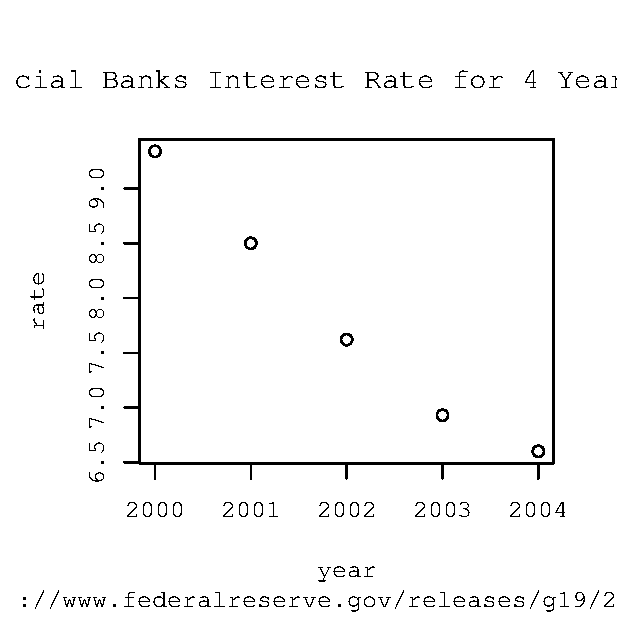
\includegraphics[width=3in]{bankRates}}
    \caption{Scatter plot of the interest rates given in Table
      \ref{table:carLoan}.}
  \label{fig:carLoan}
\end{figure}


\begin{figure}[tb]
    \centerline{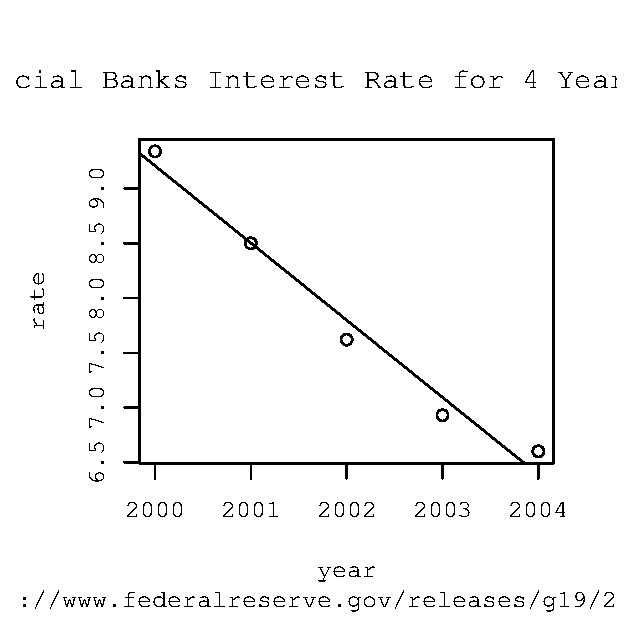
\includegraphics[width=3in]{bankRatesFit}}
    \caption{Scatter plot of the interest rates given in Table
      \ref{table:carLoan} with a linear approximation.}
  \label{fig:carLoanFit}
\end{figure}

In particular simply plugging the numbers into a software package such
as spreadsheet or specialized statistical package can show that the
data is approximated by the relationship
\begin{eqnarray*}
  \mathrm{Rate} & \approx & m (\mathrm{year}) + b, \\
  \mathrm{Rate} & \approx & -0.705 (\mathrm{year}) + 1419.208.
\end{eqnarray*}
The approximation can now be used to estimate the interest rate at
different times. For example, the interest rates can be approximated
for the years, 2002.5, 2005, 2015, and 1992:
\begin{itemize}
\item In June 2002 (2002.5) the rate is approximately 7.45\%,
\item In 2005 the rate was approximately 5.68\%,
\item In 2015 the rate will be approximately -1.36\%,
\item In 1992 the rate was approximately 14.85\%.
\end{itemize}

It is not likely that a bank will pay you to take out a loan on a car,
and the 14.85\% figure is quite high. There are some cautions that
must be observed when using straight line approximations. In
particular there is a difference between using the linear
approximation for values of the dependent variable within the sampled
observations and outside of the sampled observations. 

\begin{definition}
  A \textbf{regression line} is a straight line that is used to
  describe a linear relationship between the independent and dependent
  variables.
\end{definition}
  
\begin{definition}
  To \textbf{interpolate} is to use a regression line within the known
  values of the independent variable.
\end{definition}

\begin{definition}
  To \textbf{extrapolate} is to use a regression line outside the
  known values in the independent variable.
\end{definition}

There is another problem with the example. Part of the reason that the
correlation is so high is that the data that is examined is the result
of averaging. Each year the mean interest rate is found from all of
the banks that are observed by the US Federal Reserve and the sample
mean is reported. By examining only the mean a great deal of the
variation in the real data is lost. In Figure \ref{fig:carLoanSmear} a
set of random samples were generated. At each year a random sample was
made up whose sample mean equals the rates given in Table
\ref{table:carLoan}. Even though the sample means are the same the
correlation is reduced from the original -0.988 to -0.85. It still
demonstrates a strong linear relationship but is different from the
original reported value.

\begin{figure}[tb]
  \centerline{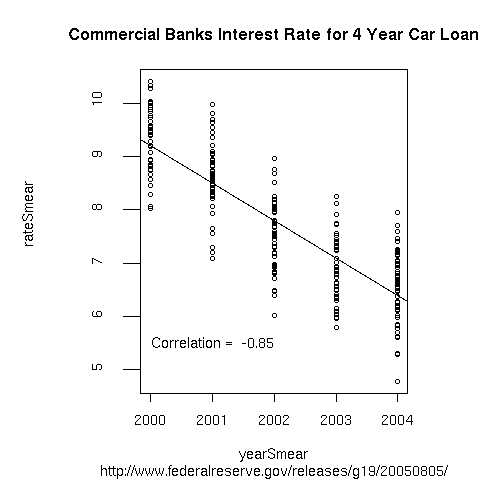
\includegraphics[height=3in]{bankRatesSmear}}
  \caption{Scatter plot of the interest rates given in Table
    \ref{table:carLoan} with extra values in each year.}
  \label{fig:carLoanSmear}
\end{figure}



\subsection{The Best Straight Line}

In the previous subsections the basic idea of a regression line is
examined.The method to find a regression line is examined using the
linear least square method. Again, it is assumed that a set of data
pairs from a set of observations has been measured, just as in
Equation (\ref{eqn:dataPairs}). The goal is to find a linear
relationship,
\begin{eqnarray*}
  y & \approx & m x + b,
\end{eqnarray*}
that gives a good description of the relationship between the data.
The goal is to find $m$ and $b$ given the data in equation
(\ref{eqn:dataPairs}).

Before the method to determine $m$ and $b$ is defined some basic
assumptions are stated. The first assumption is that the data is of
the form
\begin{eqnarray*}
  y_k & = & m x_k + b + \epsilon_k
\end{eqnarray*}
for each $k=1,\ldots,n$, and the error, $\epsilon_k$, is a random
variable. It is assumed that each random variable $\epsilon_k$ is
\begin{itemize}
\item normally distributed with mean zero and variance $\sigma^2$,
\item independent of one another (i.e. the error at the
  $k$\textsuperscript{th} observation does not depend on any other
  observation in any way.
\end{itemize}
Finally, it is assumed that the measurement of the independent
variable is done with much less error than the error made in measuring
the dependent variable. This means that the error in measuring each
$y_k$ does not depend greatly on our measurement of the corresponding
$x_k$.

The last assumption implies that the focus is on the error made
between the measurement $y_k$ and the height of the regression line,
$m x_k+b$. The error for the $k$\textsuperscript{th} observation is
\begin{eqnarray*}
  y_k - (m x_k + b).
\end{eqnarray*}
Minimizing the sum of the errors is not useful because the error
defined above can be either positive or negative, and a sum of these
errors might sum to zero and not be a good fit. The absolute value
could be used. Unfortunately, a derivative is used to minimize the
sum, and the absolute value function is not differentiable at its
minimum point.

To avoid these problems the square of each error term is used,
\begin{eqnarray*}
  \lp y_k - (m x_k + b) \rp^2.
\end{eqnarray*}
The goal is to add up all of the squares of the errors and find values
of $m$ and $b$ that make the sum of the squares of the errors as small
as possible. The sum of the squares of the errors is defined to be
\begin{eqnarray}
  \label{eqn:sse}
  \mathrm{SSE} & = & \sum_{k=1}^n \lp y_k - (m x_k + b) \rp^2.
\end{eqnarray}
It is important to note that each data pair, $(x_k,y_k)$, is a known
constant. The only variable in the expression is $m$ and $b$. 

To find the values of $m$ and $b$ that minimizes the SSE the
respective derivatives are set equal to zero. First, the derivative of
SSE with respect to $m$ must be zero,
\begin{eqnarray*}
  0 & = & \frac{\partial}{\partial m} SSE, \\
  & = & \sum_{k=1}^n 2\lp y_k - (m x_k + b) \rp (-x_k), \\
  & = & -2 \sum_{k=1}^n (x_k y_k) + 
  2 m \sum_{k=1}^n x_k^2 + 2 b \sum_{k=1}^n x_k.
\end{eqnarray*}
An equivalent expression is
\begin{eqnarray}
  \label{eqn:gradientSSEm}
  m \sum_{k=1}^n x_k^2 + b \sum_{k=1}^n x_k & = & 
  \sum_{k=1}^n (x_k y_k),
\end{eqnarray}
where $m$ and $b$ are unknowns, but the sums represent known
constants.

Second the derivative of SSE with respect to $b$ must be zero,
\begin{eqnarray*}
  0 & = & \frac{\partial}{\partial b} SSE, \\
  & = & \sum_{k=1}^n 2\lp y_k - (m x_k + b) \rp (-1), \\
  & = & -2 \sum_{k=1}^n y_k + 
  2 m \sum_{k=1}^n x_k + 2 b \sum_{k=1}^n 1.
\end{eqnarray*}
An equivalent expression is
\begin{eqnarray}
  \label{eqn:gradientSSEb}
  m \sum_{k=1}^n x_k + n\,b & = & 
  \sum_{k=1}^n y_k.
\end{eqnarray}
Equations (\ref{eqn:gradientSSEm}) and (\ref{eqn:gradientSSEb})
represent two equations and two unknowns, and the values of $m$ and
$b$ can be calculated using standard techniques. (See the assignments
at the end of this subsection.)

\begin{assignment}
  Express equations (\ref{eqn:gradientSSEm}) and
  (\ref{eqn:gradientSSEb}) in matrix form,
  \begin{eqnarray*}
    B 
    \left[
      \begin{array}{rr}
        m \\ b
      \end{array}
      \right] & = & \vec{b}.
  \end{eqnarray*}
  (i.e. find the entries in the matrix $B$ and vector $\vec{b}$.) Find
  the solution of the linear system using Cramer's rule.
\end{assignment}

\if y\solutions
\textbf{Solution:} 

Equations (\ref{eqn:gradientSSEm}) and (\ref{eqn:gradientSSEb}) are
the following:
\begin{eqnarray}
  m \sum_{k=1}^n x_k^2 + b \sum_{k=1}^n x_k & = & 
  \sum_{k=1}^n (x_k y_k), \\
  m \sum_{k=1}^n x_k + n\,b & = & 
  \sum_{k=1}^n y_k.
\end{eqnarray}
Here the unknowns are $m$ and $b$, and the vector of unknowns is
\begin{eqnarray*}
  \left[
    \begin{array}{rr}
      m \\ b
    \end{array}
  \right].
\end{eqnarray*}
Writing the equations in vector/matrix form yields
\begin{eqnarray*}
  \left[
    \begin{array}{rr}
      \sum_{k=1}^n x_k^2  & \sum_{k=1}^n x_k \\
      \sum_{k=1}^n x_k & n
    \end{array}
  \right]
  \left[
    \begin{array}{rr}
      m \\ b
    \end{array}
  \right] & = & 
  \left[
    \begin{array}{rr}
      \sum_{k=1}^n (x_k y_k) \\ \sum_{k=1}^n y_k
    \end{array}
  \right].
\end{eqnarray*}

The value for $m$ can be found using Cramer's rule,
\begin{eqnarray*}
  m & = & \frac{
    \det \left[
    \begin{array}{rr}
      \sum_{k=1}^n (x_k y_k) & \sum_{k=1}^n x_k \\
      \sum_{k=1}^n y_k & n
    \end{array}
  \right]
  }{
    \det \left[
    \begin{array}{rr}
      \sum_{k=1}^n x_k^2  & \sum_{k=1}^n x_k \\
      \sum_{k=1}^n x_k & n
    \end{array}
  \right]
}, \\
& = & \frac{
  n \sum_{k=1}^n (x_k y_k) - \lp \sum_{k=1}^n x_k \rp \lp \sum_{k=1}^n y_k \rp}{
  n \sum_{k=1}^n x_k^2 - \lp \sum_{k=1}^n x_k \rp^2}.
\end{eqnarray*}


Likewise, the value of $b$ can also be found using Cramer's rule,
\begin{eqnarray*}
  b & = & \frac{
\det \left[
    \begin{array}{rr}
      \sum_{k=1}^n x_k^2  &  \sum_{k=1}^n (x_k y_k)  \\
      \sum_{k=1}^n x_k & \sum_{k=1}^n y_k
    \end{array}
  \right]
    }{\det \left[
    \begin{array}{rr}
      \sum_{k=1}^n x_k^2  & \sum_{k=1}^n x_k \\
      \sum_{k=1}^n x_k & n
    \end{array}
  \right]}, \\
& = & \frac{\lp\sum_{k=1}^n x_k^2\rp\lp\sum_{k=1}^n y_k\rp
  - \lp\sum_{k=1}^n (x_k y_k)\rp\lp\sum_{k=1}^n x_k\rp
}{n \sum_{k=1}^n x_k^2 - \lp \sum_{k=1}^n x_k \rp^2}.
\end{eqnarray*}

\fi

\begin{assignment}
  Define a matrix
  \begin{eqnarray*}
    A & = & 
    \left[
      \begin{array}{rr}
        x_1 & 1 \\
        x_2 & 1 \\
        x_3 & 1 \\
        \vdots & \vdots \\
        x_n & 1
      \end{array}
    \right],
  \end{eqnarray*}
  and a vector 
  \begin{eqnarray*}
    \vec{y} & = & 
    \left[
      \begin{array}{r}
        y_1 \\
        y_2 \\
        y_3 \\
        \vdots  \\
        y_n 
      \end{array}
    \right].
  \end{eqnarray*}
  Show that the system of equations in the previous assignment can be
  written equivalently as
  \begin{eqnarray*}
    A^T A
    \left[
      \begin{array}{rr}
        m \\ b
      \end{array}
      \right] & = & A^T \vec{y}.
  \end{eqnarray*}
\end{assignment}

\if y\solutions
\textbf{Solution:} 

The matrix $A^TA$ is given by
\begin{eqnarray*}
      \left[
      \begin{array}{rrrrr}
        x_1 & x_2 & x_3 & \cdots & x_n  \\
        1   & 1   & 1   & \cdots & 1
      \end{array}
    \right]^T
    \left[
      \begin{array}{rr}
        x_1 & 1 \\
        x_2 & 1 \\
        x_3 & 1 \\
        \vdots & \vdots \\
        x_n & 1
      \end{array}
    \right]
    & = & 
    \left[
      \begin{array}{rr}
        \sum^n_{k=1} x_k^2 & \sum^n_{k=1} x_k \\
        \sum^n_{k=1} x_k & n
      \end{array}
    \right].
\end{eqnarray*}
This is the same as the matrix $B$ defined in the previous
assignment. 

The matrix $A^T\vec{y}$ is  given by
\begin{eqnarray*}
      \left[
      \begin{array}{rrrrr}
        x_1 & x_2 & x_3 & \cdots & x_n  \\
        1   & 1   & 1   & \cdots & 1
      \end{array}
    \right]^T
      \left[
      \begin{array}{r}
        y_1 \\
        y_2 \\
        y_3 \\
        \vdots  \\
        y_n 
      \end{array}
    \right] & = & 
    \left[
      \begin{array}{r}
        \sum^n_{k=1} x_k y_k \\ \sum^n_{k=1} y_k
      \end{array}
    \right].
\end{eqnarray*}
This is the same as the vector $\vec{b}$ defined in the previous assignment.

\fi


%\subsection{Analysis of Variance (Advanced Topic)}


\bibliographystyle{siam}
\bibliography{statistics}




\end{document}

% LocalWords:  Cavendish's roman SSE Ziamandanis protractors photocells

